\chapter{Generazione del Bytecode Kitten}\label{chap:translate}
%
\vspace*{-2ex}
\begin{center}

\includegraphics[width=6.5cm]{cat9.jpg}
\end{center}
%\vspace*{-2ex}
%
L'analisi semantica del Capitolo~\ref{chap:semantical} ha garantito che
il codice Kitten non contenga alcun errore semantico. Ha inoltre
annotato l'albero di sintassi astratta con informazioni relative
al tipo statico delle espressioni che vi occorrono; gli accessi a
campi, costruttori e metodi con la specifica dichiarazione
del campo, costruttore
o metodo a cui fanno riferimento. Siamo ora nelle condizioni di
generare del codice \emph{intermedio}, \cioe indipendente dall'architettura
verso la quale stiamo compilando, ma pensato piuttosto per essere
facilmente sintetizzabile a partire dall'albero di sintassi astratta
e facilmente ottimizzabile. Esso verr\`a poi traslato in codice oggetto,
specifico all'architettura verso cui compiliamo.
Il codice intermedio che useremo \`e il \emph{bytecode Kitten}, che pu\`o
essere visto come una versione semplificata ed esplicitamente tipata del
\emph{Java bytecode}.
%
\section{Il bytecode Kitten}
%
Il bytecode Kitten \`e un linguaggio di programmazione pensato per
essere eseguito da una macchina astratta che ha a disposizione:
%
\begin{enumerate}
\item un insieme di \emph{variabili locali}, potenzialmente illimitato, che
      possono contenere valori primitivi o riferimenti a oggetti o array;
\item uno stack di variabili temporanee, detto \emph{stack degli operandi},
      potenzialmente illimitato, che pu\`o contenere valori primitivi o
      riferimenti a oggetti o array;
\item uno \emph{stack di attivazione}, formato da un numero potenzialmente
      illimitato di \emph{frame di attivazione} di metodi. Ciascun frame
      di attivazione contiene le variabili locali e lo stack di attivazione
      di un metodo;
\item una \emph{memoria} o \emph{heap}, che contiene oggetti e array
      allocati dinamicamente dal programma in esecuzione.
\end{enumerate}

La maggior parte delle istruzioni del bytecode Kitten operano sulle
variabili locali e sullo stack degli operandi. Un numero limitato
(invocazione e ritorno da metodo) operano anche sullo stack di attivazione.
Le sole operazioni che operano sulla memoria sono quelle
di creazione di oggetto o array e di accesso a campi o array.
%
\begin{figure}[t]
\begin{verbatim}
      Led():                                    isOn():
        return void                               load 0 of type Led
                                                  getfield Led.state
      on():                                       return boolean
        load 0 of type Led
        const true                              isOff():
        putfield Led.state                        load 0 of type Led
        return void                               getfield Led.state
                                                  neg boolean
      off():                                      return boolean
        load 0 of type Led
        const false
        putfield Led.state
        return void
\end{verbatim}
\caption{La compilazione in bytecode Kitten dei metodi della classe \texttt{Led} in Figura~\ref{fig:led}.}\label{fig:led_bytecode}
\end{figure}

Si consideri la Figura~\ref{fig:led_bytecode}. Essa mostra la compilazione
in bytecode Kitten dei metodi della classe \texttt{Led} in
Figura~\ref{fig:led}. All'inizio dell'esecuzione di un metodo o costruttore,
lo stack degli operandi \`e vuoto e le variabili locali contengono i
parametri attuali del metodo o costruttore. In particolare, la variabile
locale numero $0$ contiene sempre il riferimento all'oggetto corrente,
\cioe quello che nel codice sorgente sarebbe stato \texttt{this}, che \e
un parametro implicito in tutte le chiamate di metodo o costruttore. La
variabile locale $1$ contiene il primo parametro attuale esplicito,
la variabile locale $2$ il secondo parametro attuale esplicito, e \cosi via.
Si noti comunque che le variabili locali possono essere usate anche per
contenere vere e proprie variabili locali ai metodi e non solo per contenere
i parametri attuali. Nell'esempio
in Figura~\ref{fig:led_bytecode}, solo la variabile locale $0$ \`e utilizzata,
dal momento che nessun metodo richiede dei parametri espliciti \nec
variabili locali.
L'istruzione \texttt{load 0 of type Led}
indica di copiare il riferimento all'oggetto corrente in cima allo
stack degli operandi. L'istruzione \texttt{const} serve invece a caricare
in cima allo stack degli operandi una costante. Nella
Figura~\ref{fig:led_bytecode} si tratta di una costante booleana.
Le istruzioni \texttt{getfield} e \texttt{putfield} servono, rispettivamente,
a leggere e a scrivere un campo di un oggetto. L'istruzione \texttt{neg}
nega il valore che sta in cima allo stack degli operandi. L'istruzione
\texttt{return} termina l'esecuzione di un metodo o costruttore ritornando
possibilmente un valore al chiamante.

\begin{figure}[t]
\begin{center}
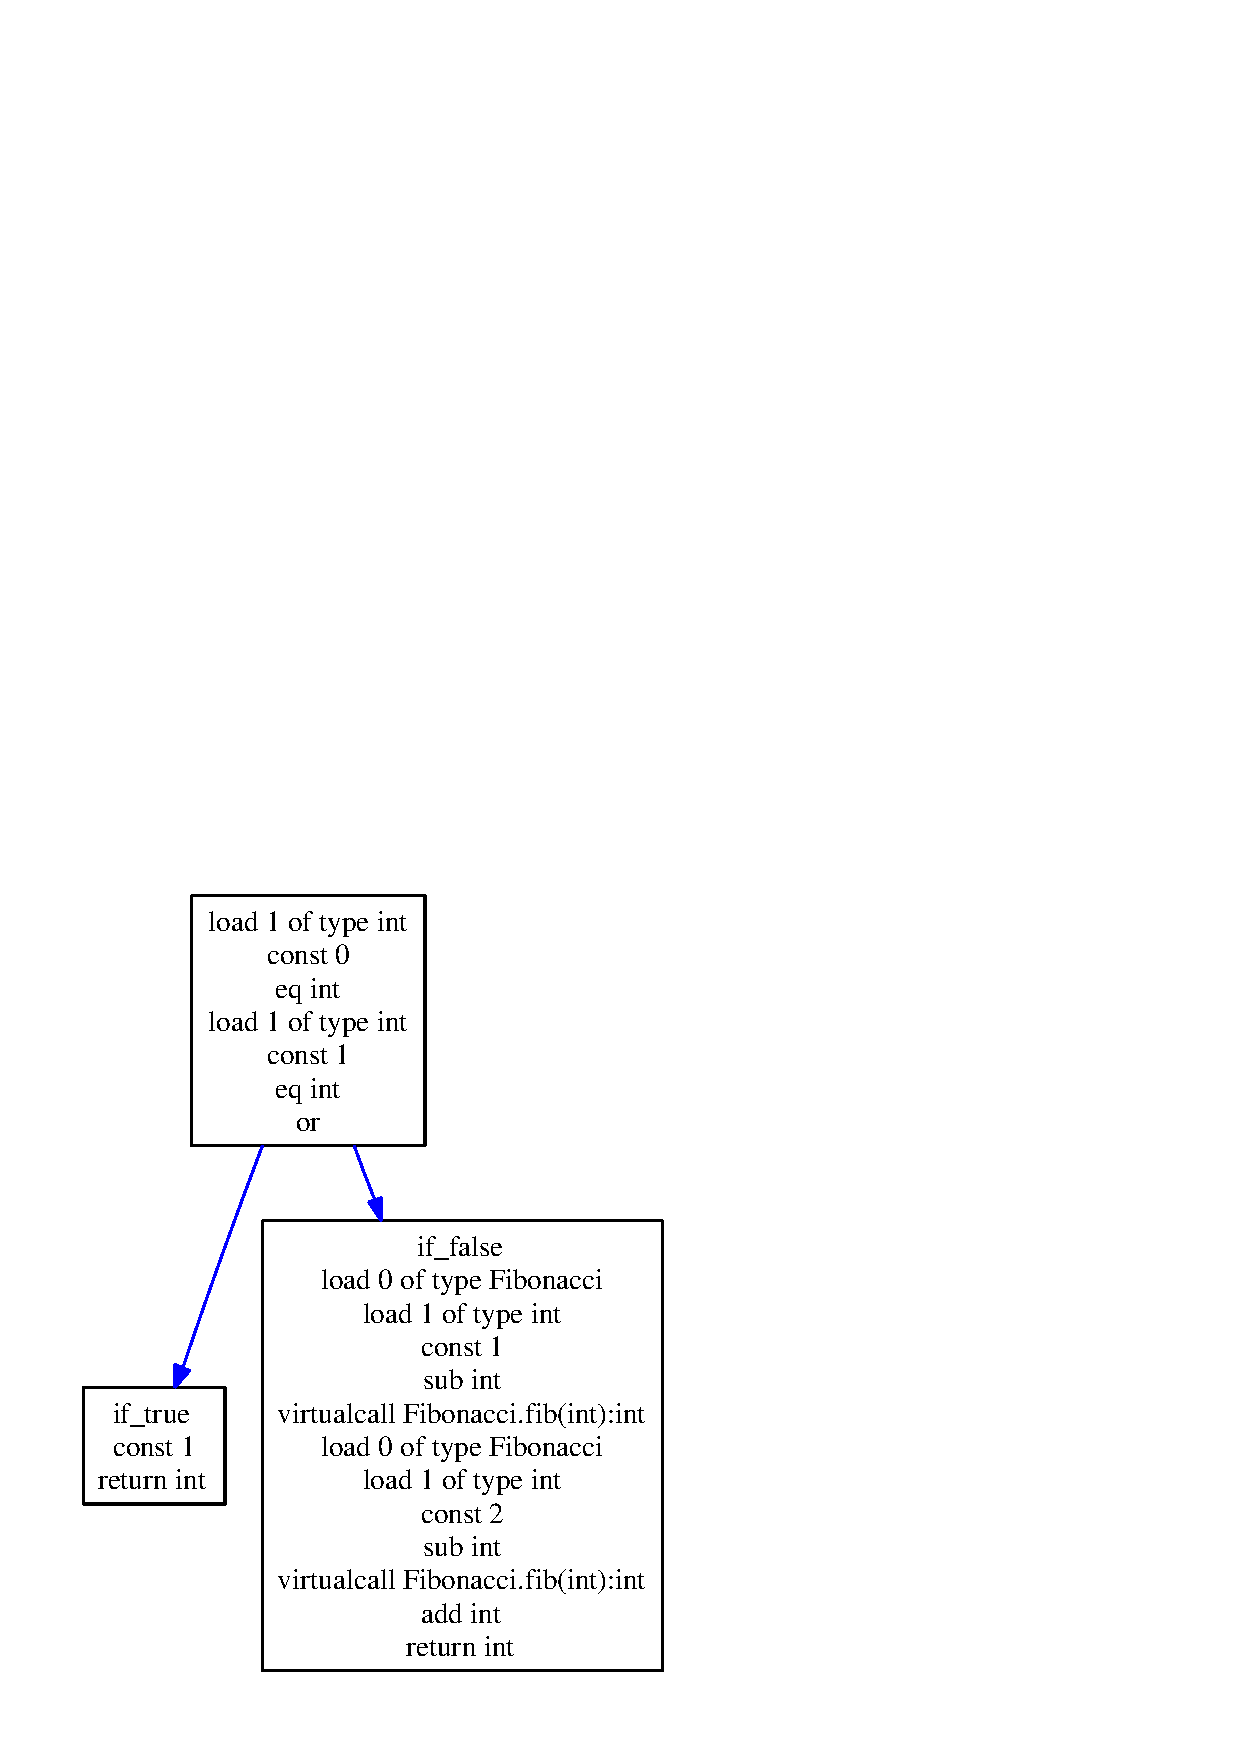
\epsfig{file = fib.pdf, width = 8cm}
\end{center}
\caption{La compilazione in bytecode Kitten del metodo \texttt{fib()} in Figura~\ref{fig:fibonacci}.}\label{fig:fib_bytecode}
\end{figure}
%
Il bytecode in Figura~\ref{fig:led_bytecode} ha una struttura di controllo
particolarmente semplice, dal momento che non prevede condizionali \nec cicli.
La Figura~\ref{fig:fib_bytecode} mostra un esempio \piu complesso:
la compilazione in bytecode Kitten del metodo \texttt{fib()} in
Figura~\ref{fig:fibonacci}. La presenza di un comando condizionale in
Figura~\ref{fig:fibonacci} diventa un'alternativa di controllo nel
bytecode Kitten in Figura~\ref{fig:fib_bytecode}: il risultato dell'istruzione
\texttt{or} determina l'istradamento del controllo verso il ramo
\texttt{if\_true} o verso quello \texttt{if\_false}.

L'esempio precedente mostra che il bytecode Kitten \`e in effetti un grafo
di \emph{blocchi di codice} che contengono codice
sequenziale. Un ulteriore esempio \`e la compilazione del ciclo:
%
\begin{verbatim}
  for (int i := 0; i < 5; i := i + 1) {}
\end{verbatim}
%
mostrata in Figura~\ref{fig:cycle_bytecode}. Questa volta
l'istradamento del controllo dipende dal risultato di un confronto.
In particolare, il confronto fra la variabile locale $1$, che contiene
la variabile \texttt{i} del ciclo, e la costante intera $5$ determina
l'istradamento del codice verso il ramo \texttt{if\_cmplt}
(\emph{IF the CoMParison is Less Than}) o verso quello
\texttt{if\_cmpge} (\emph{IF the CoMParison is Greater than or Equal}).
%
\begin{figure}[t]
\begin{center}
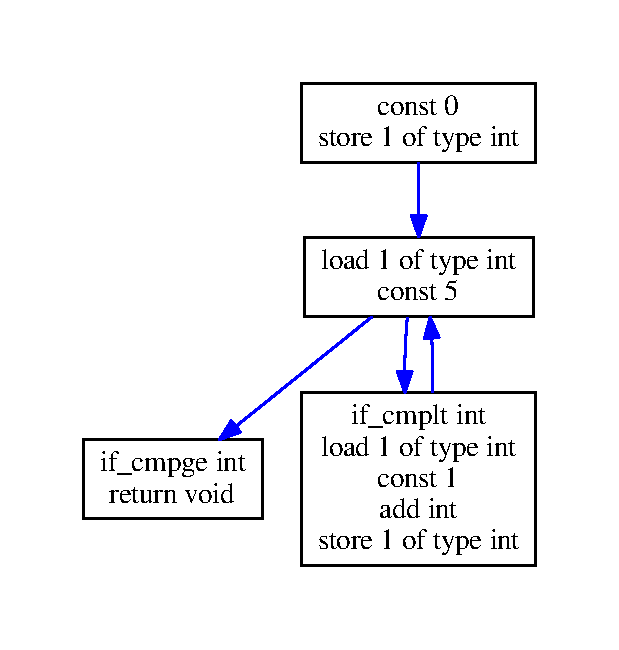
\epsfig{file = ciclo.pdf, width = 8cm}
\end{center}
\caption{La compilazione in bytecode Kitten di un ciclo \texttt{for}.}\label{fig:cycle_bytecode}
\end{figure}
%
\subsection{Le istruzioni sequenziali}\label{subsec:sequential_bytecodes}
%
\begin{figure}
\begin{center}
\begin{tabular}{|c|}
\hline\mbox{}\\
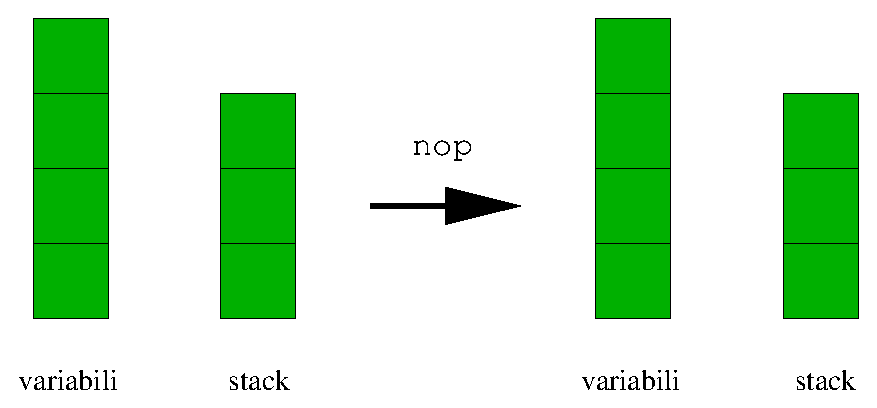
\epsfig{file = bytecodes/nop.eps, width = 12cm}\\\hline
\mbox{}\\
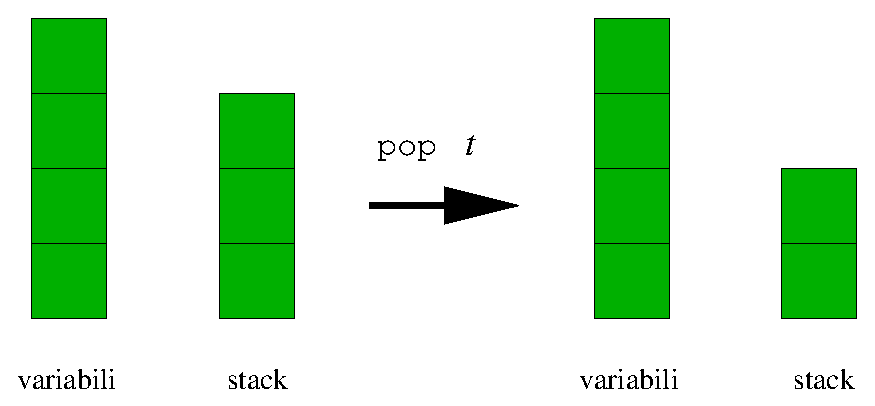
\epsfig{file = bytecodes/pop.eps, width = 12cm}\\\hline
\mbox{}\\
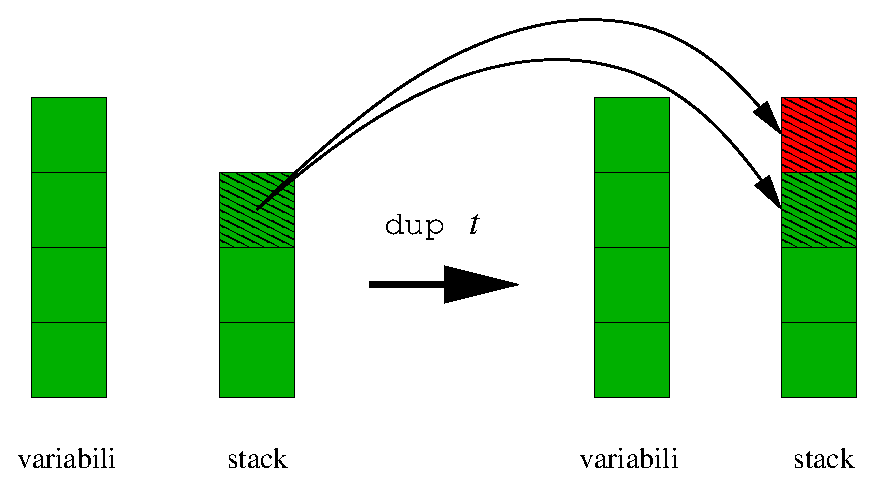
\epsfig{file = bytecodes/dup.eps, width = 12cm}\\\hline
\end{tabular}
\end{center}
\caption{Le istruzioni \texttt{nop}, \texttt{pop} e \texttt{dup} del bytecode Kitten.}
  \label{fig:bytecodes1}
\end{figure}
%
\begin{figure}
\begin{center}
\begin{tabular}{|c|}
\hline\mbox{}\\
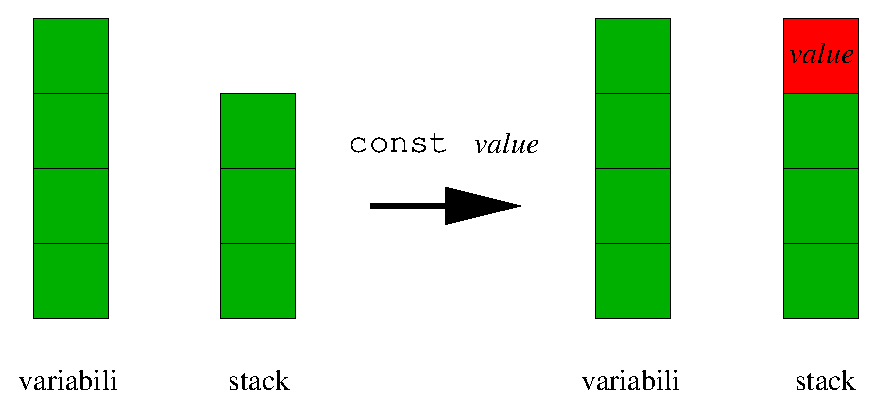
\epsfig{file = bytecodes/const.eps, width = 12cm}\\\hline
\hline\mbox{}\\
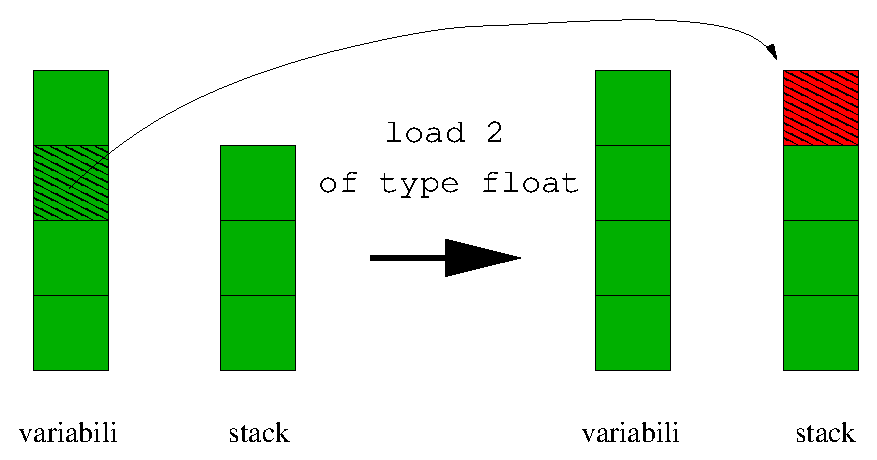
\epsfig{file = bytecodes/load.eps, width = 12cm}\\\hline
\mbox{}\\
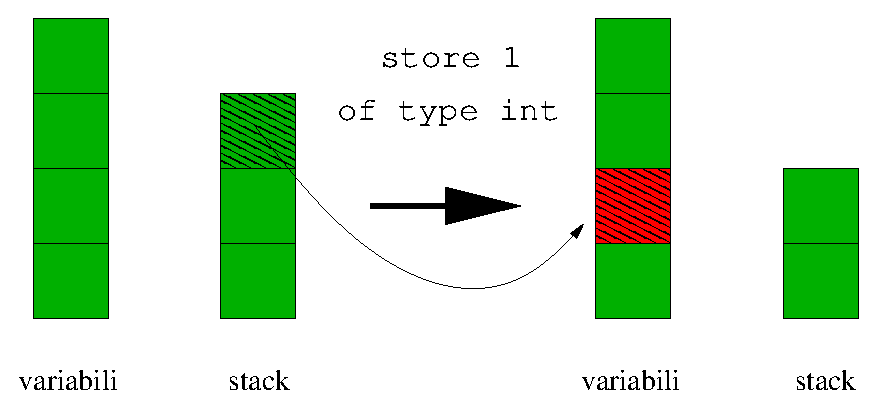
\epsfig{file = bytecodes/store.eps, width = 12cm}\\\hline
\end{tabular}
\end{center}
\caption{Le istruzioni \texttt{const}, \texttt{load} e \texttt{store} del bytecode Kitten.}
  \label{fig:bytecodes2}
\end{figure}
%
\begin{figure}
\begin{center}
\begin{tabular}{|c|}
\hline\mbox{}\\
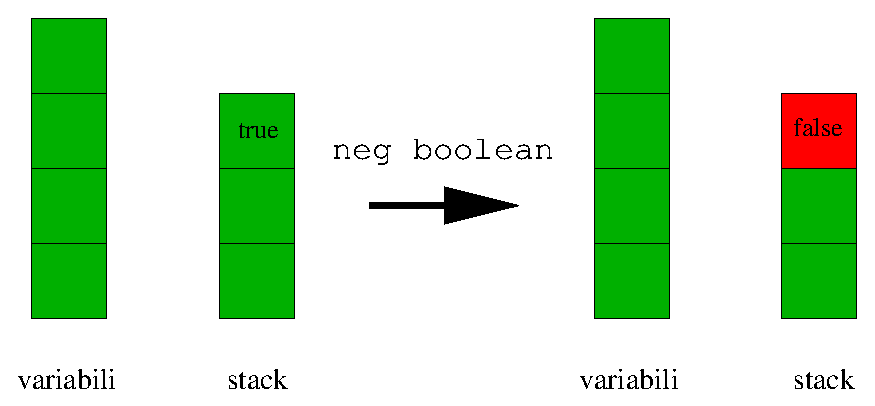
\epsfig{file = bytecodes/neg.eps, width = 12cm}\\\hline
\mbox{}\\
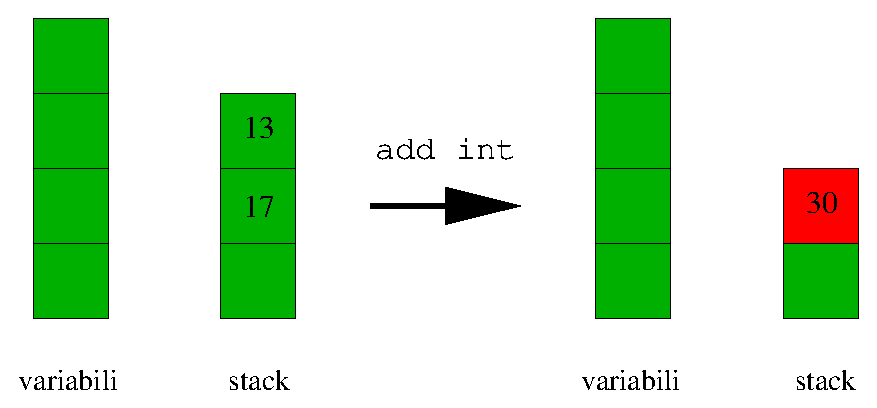
\epsfig{file = bytecodes/add.eps, width = 12cm}\\\hline
\mbox{}\\
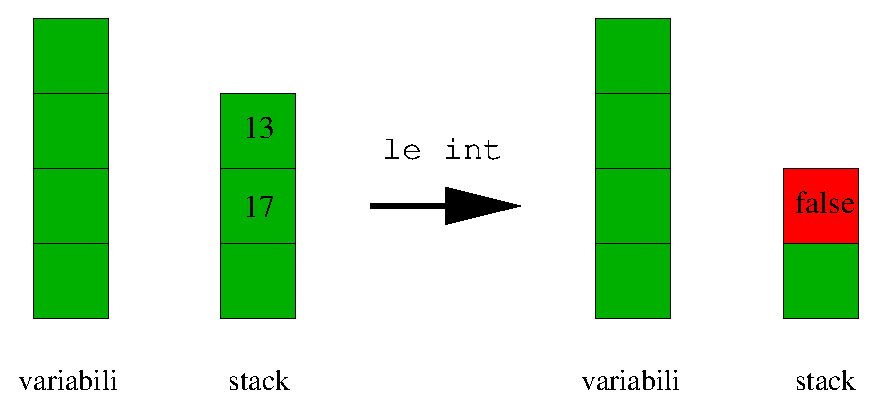
\epsfig{file = bytecodes/le.eps, width = 12cm}\\\hline
\end{tabular}
\end{center}
\caption{Le istruzioni \texttt{neg}, \texttt{add} e \texttt{le} del bytecode Kitten.}
  \label{fig:bytecodes3}
\end{figure}
%
\begin{figure}
\begin{center}
\begin{tabular}{|c|}
\hline\mbox{}\\
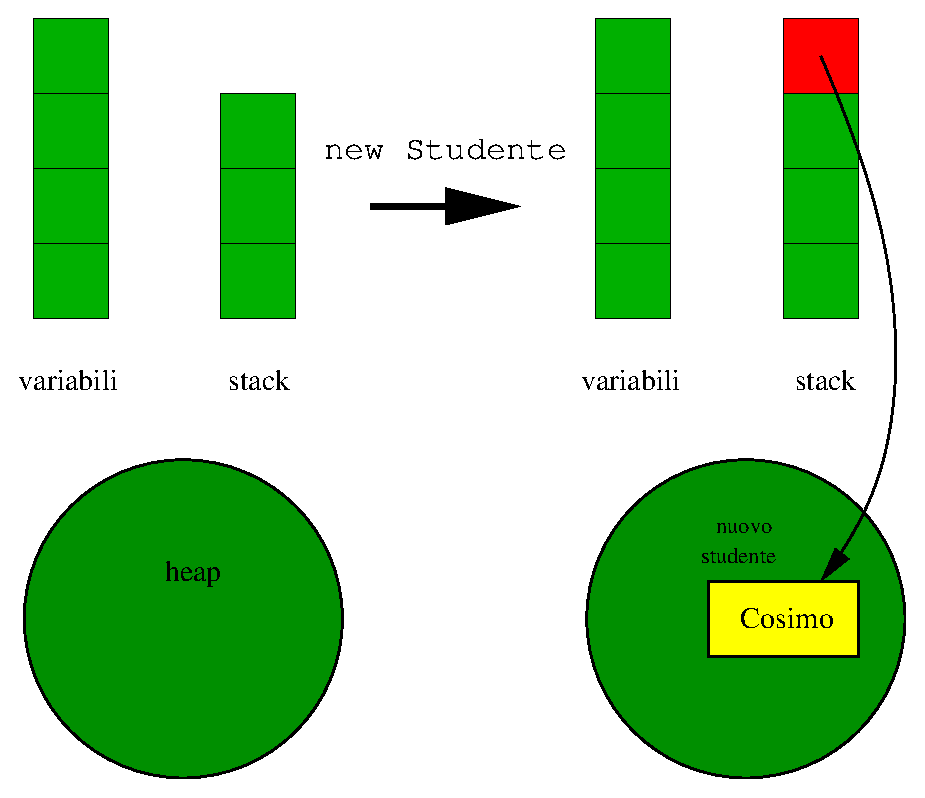
\epsfig{file = bytecodes/new.eps, width = 11.5cm}\\\hline
\mbox{}\\
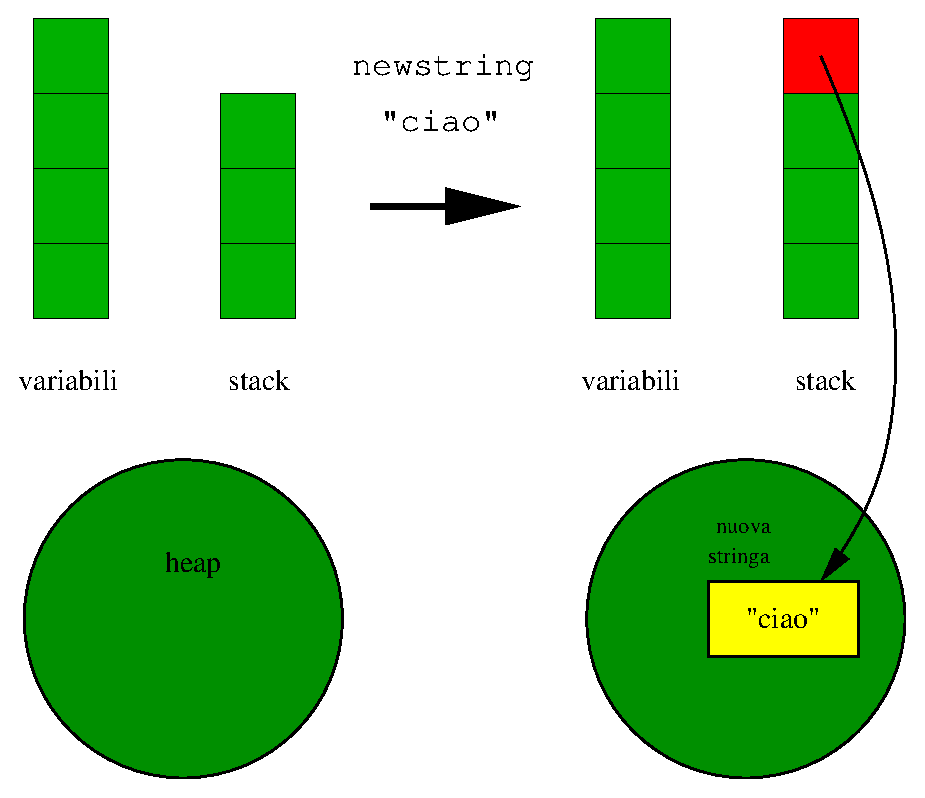
\epsfig{file = bytecodes/newstring.eps, width = 11.5cm}\\\hline
\end{tabular}
\end{center}
\caption{Le istruzioni \texttt{new} e \texttt{newstring} del bytecode Kitten.}
  \label{fig:bytecodes4}
\end{figure}
%
\begin{figure}
\begin{center}
\begin{tabular}{|c|}
\hline\mbox{}\\
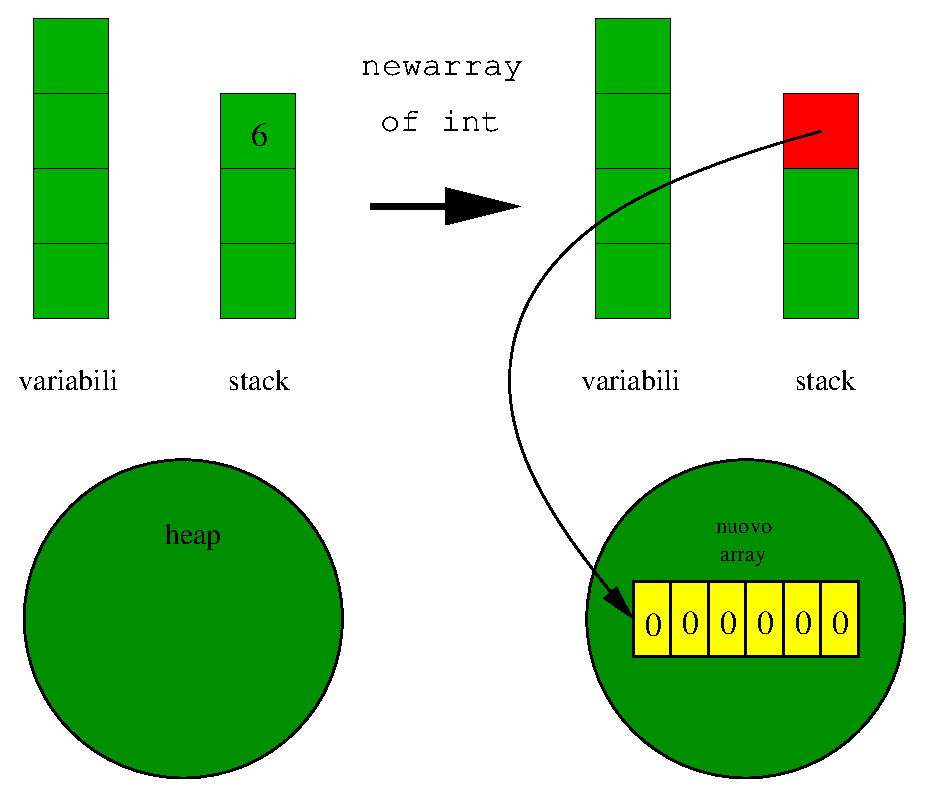
\epsfig{file = bytecodes/newarray.eps, width = 11.3cm}\\\hline
\mbox{}\\
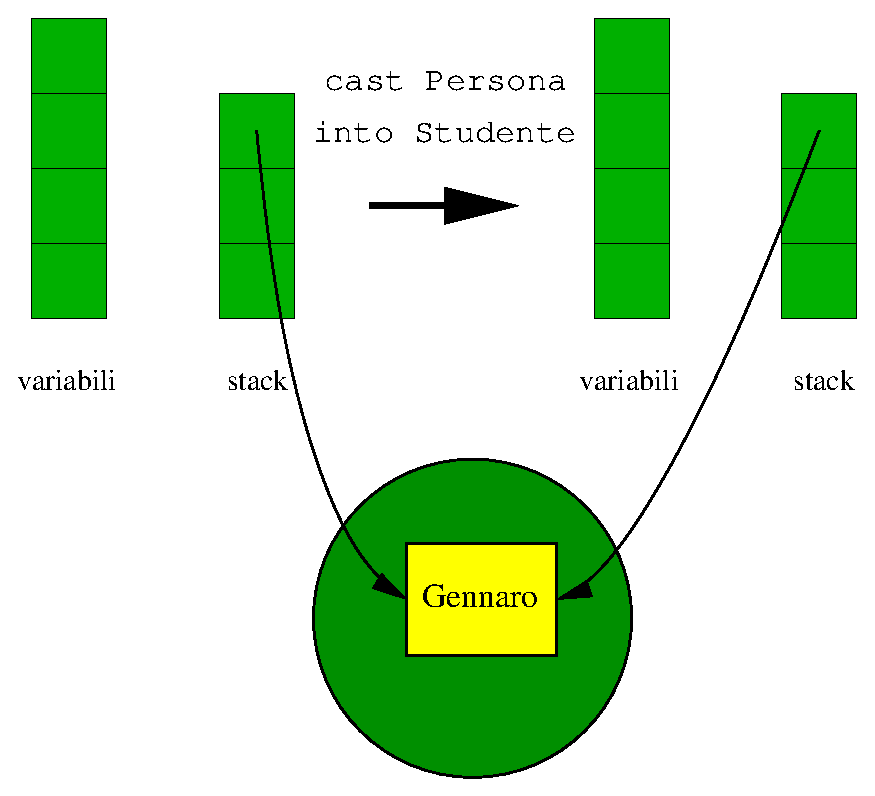
\epsfig{file = bytecodes/cast.eps, width = 11.3cm}\\\hline
\end{tabular}
\end{center}
\caption{Le istruzioni \texttt{newarray} e \texttt{cast} del bytecode Kitten.}
  \label{fig:bytecodes5}
\end{figure}
%
\begin{figure}
\begin{center}
\begin{tabular}{|c|}
\hline\mbox{}\\
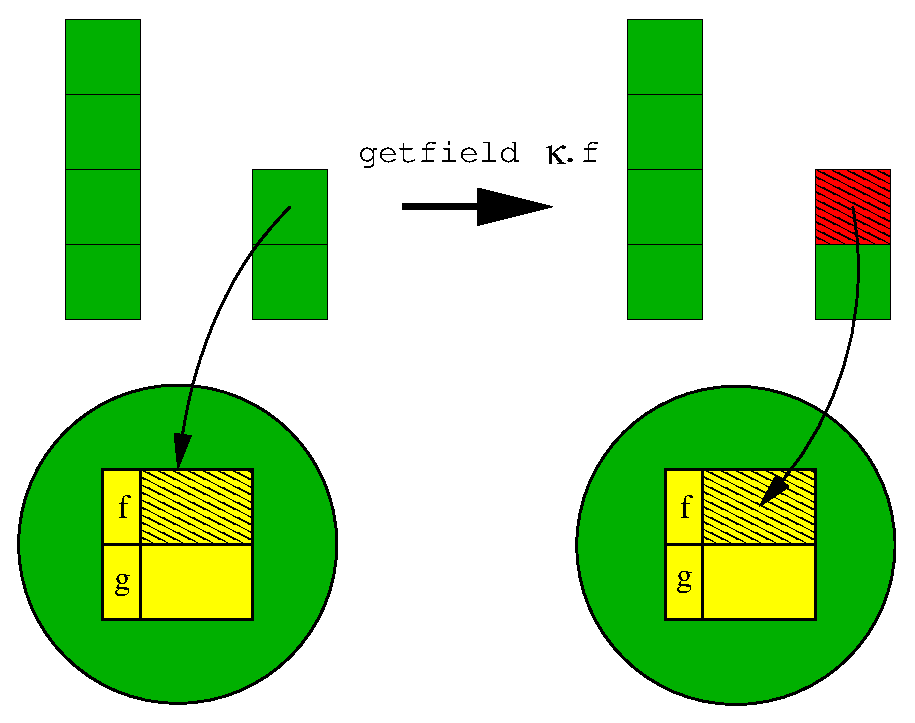
\epsfig{file = bytecodes/getfield.eps, width = 12cm}\\\hline
\mbox{}\\
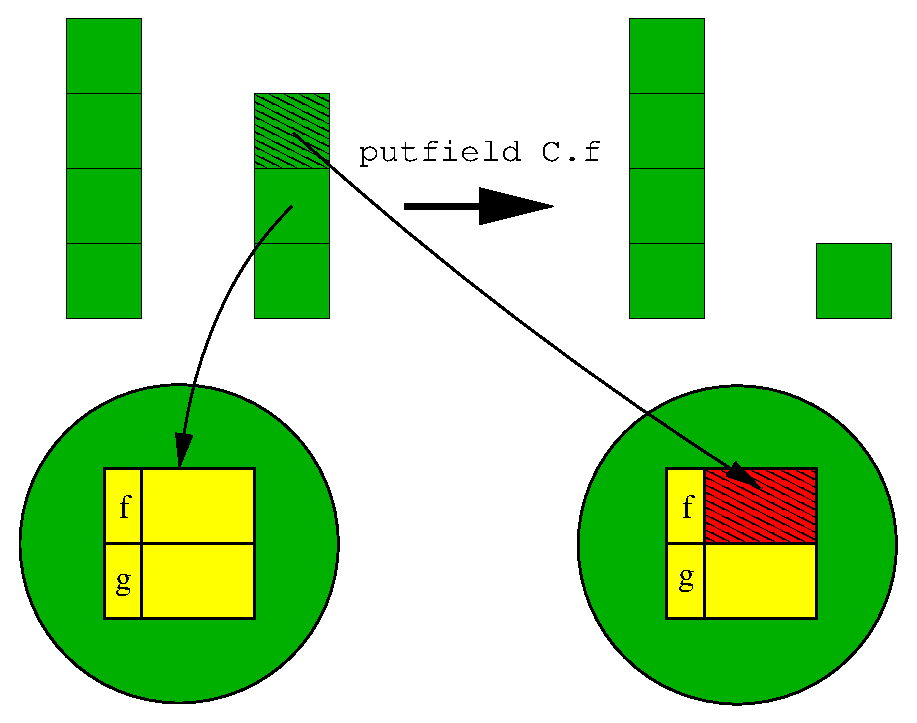
\epsfig{file = bytecodes/putfield.eps, width = 12cm}\\\hline
\end{tabular}
\end{center}
\caption{Le istruzioni \texttt{getfield} e \texttt{putfield} del bytecode Kitten.}
  \label{fig:bytecodes6}
\end{figure}
%
\begin{figure}
\begin{center}
\begin{tabular}{|c|}
\hline\mbox{}\\
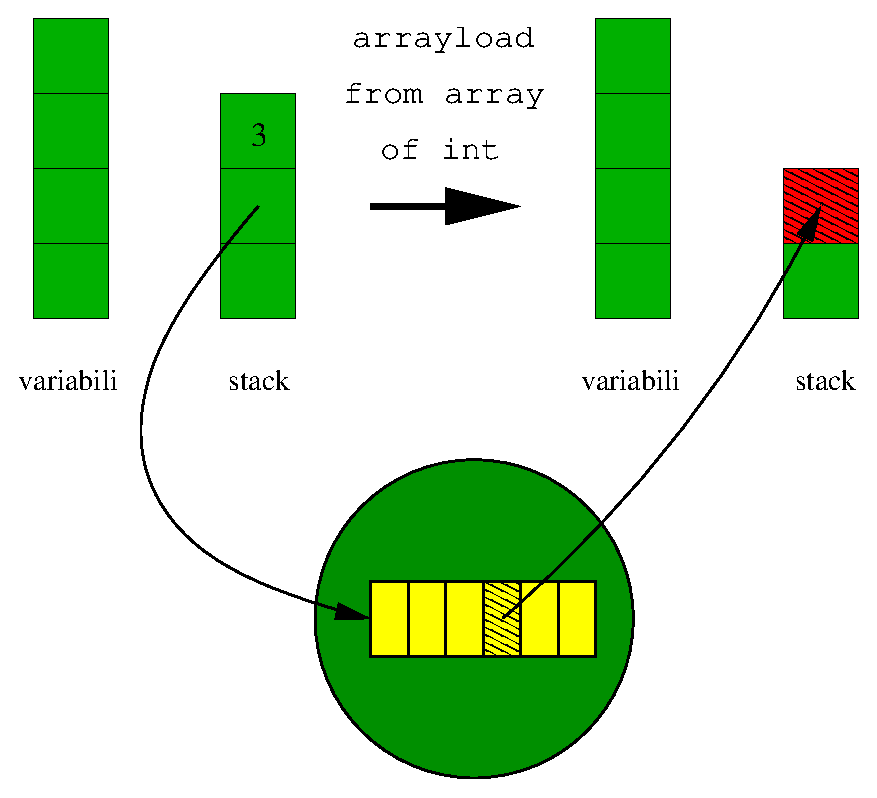
\epsfig{file = bytecodes/arrayload.eps, width = 11.3cm}\\\hline
\mbox{}\\
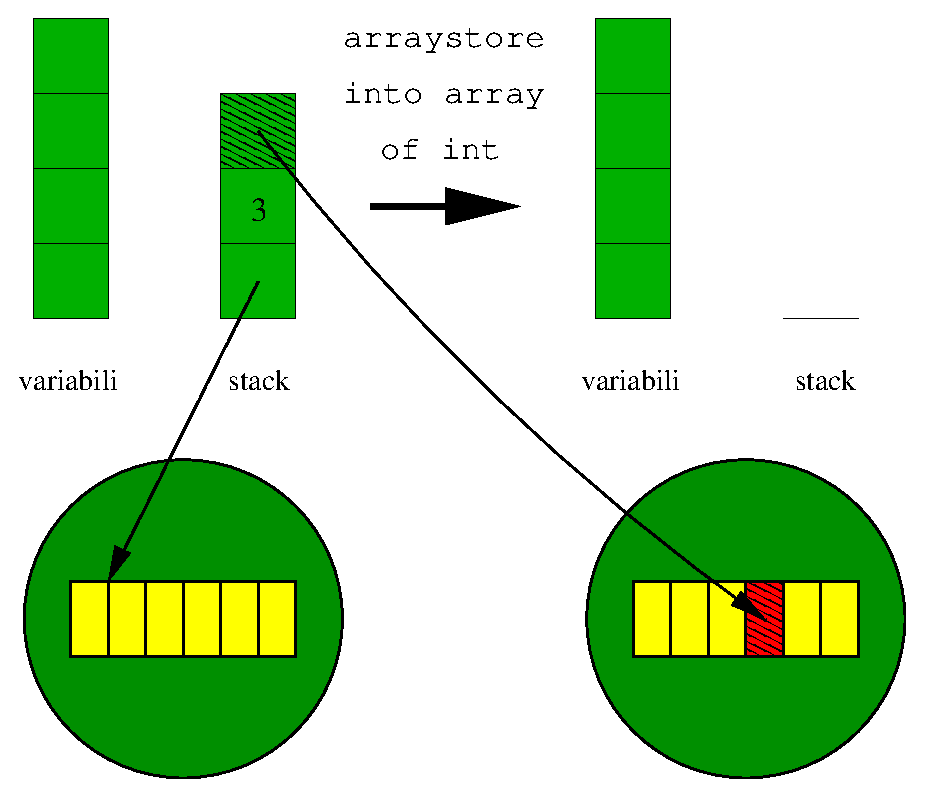
\epsfig{file = bytecodes/arraystore.eps, width = 11.3cm}\\\hline
\end{tabular}
\end{center}
\caption{Le istruzioni \texttt{arrayload} e \texttt{arraystore} del bytecode Kitten.}
  \label{fig:bytecodes7}
\end{figure}
%
\begin{figure}
\begin{center}
\begin{tabular}{|c|}
\hline\mbox{}\\
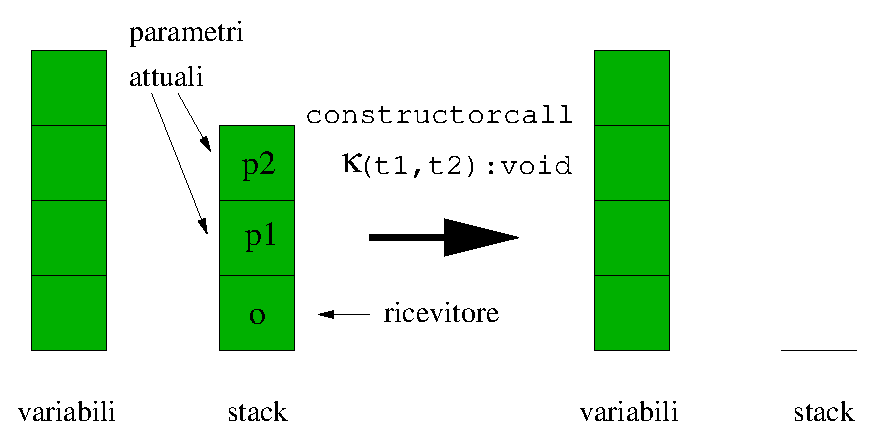
\epsfig{file = bytecodes/constructorcall.eps, width = 12cm}\\\hline
\mbox{}\\
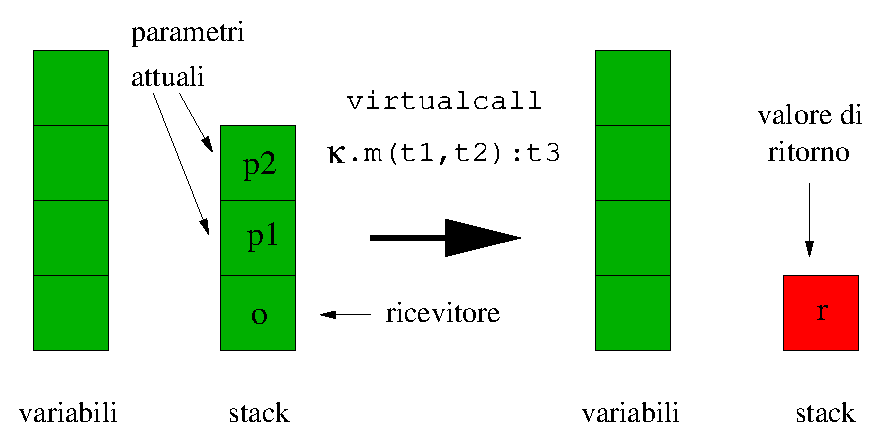
\epsfig{file = bytecodes/virtualcall.eps, width = 12cm}\\\hline
\mbox{}\\
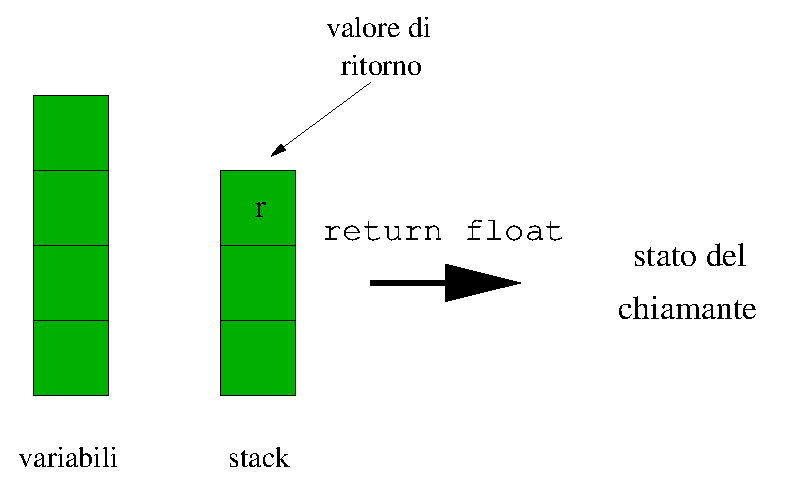
\epsfig{file = bytecodes/return.eps, width = 12cm}\\\hline
\end{tabular}
\end{center}
\caption{Le istruzioni \texttt{constructorcall}, \texttt{virtualcall} e \texttt{return} del bytecode Kitten.}
  \label{fig:bytecodes8}
\end{figure}

Esaminiamo adesso il set di istruzioni messe a disposizione dal bytecode
Kitten. Per ognuna di esse mostriamo il suo effetto sulle variabili locali,
sullo stack degli operandi e sulla memoria o heap. Dal momento che
poche istruzioni operano sullo heap, nelle figure lo indicheremo solo per quelle poche
istruzioni per cui esso \`e effettivamente significativo.
Le istruzioni del bytecode Kitten
sono \emph{tipate}, nel senso che \e specificato il tipo
degli operandi su cui possono operare. Esse non effettuano mai una promozione
di tipo per cui, quando nella loro descrizione useremo il termine
\emph{sottotipo}, esso va inteso nel senso dell'operazione
\texttt{canBeAssignedToSpecial()} della Sezione~\ref{sec:semantical_types}.
%
\begin{description}
\item[\underline{$\mathtt{nop}$}.] Questa istruzione non modifica in nulla
  lo stato della macchina astratta. L'effetto della sua esecuzione pu\`o
  quindi essere rappresentato come in Figura~\ref{fig:bytecodes1}.
\item[\underline{$\mathtt{pop}$ $t$}.]
  Rimuove la cima dello stack degli operandi, che deve avere tipo $t$
  (Figura~\ref{fig:bytecodes1}).
\item[\underline{$\mathtt{dup}$ $t$}.] Duplica il valore in cima allo stack
  (Figura~\ref{fig:bytecodes1}) che deve avere tipo $t$.
  Si noti che se tale valore fosse un
  riferimento a un oggetto o a un array allora verrebbe duplicato il
  riferimento, creandone un alias, non l'oggetto o l'array.
\item[\underline{$\mathtt{const}\ \mathit{value}$}.]
  Carica in cima allo stack un valore
  costante (Figura~\ref{fig:bytecodes2}).
  \`E possibile caricare valori booleani, interi, float e la
  costante \texttt{nil}.
\item[\underline{$\mathtt{load\ \mathit{l}\ of\ type\ \mathit{t}}$}.]
  Carica in cima allo stack degli operandi
  una copia del valore della variabile locale
  numero $l$, che deve contenere un valore di tipo $t$
  (Figura~\ref{fig:bytecodes2}).
\item[\underline{$\mathtt{store\ \mathit{l}\ of\ type\ \mathit{t}}$}.]
  Sposta dentro la variabile locale numero $l$ il valore che si trova
  in cima allo stack degli operandi. La cima di tale stack deve contenere un
  valore del tipo $t$ e viene rimossa dall'operazione
  (Figura~\ref{fig:bytecodes2}).
\item[\underline{$\mathtt{neg\ \mathit{t}}$}.]
  Nega il valore in cima allo stack degli operandi
  (Figura~\ref{fig:bytecodes3}). Tale valore deve
  essere di tipo $t$. \`E possibile che $t$ sia \texttt{boolean},
  \texttt{int} o \texttt{float}. Si noti che il valore in cima allo
  stack che viene usato per calcolare l'operazione \texttt{neg} scompare
  dallo stack e viene sostituito dal risultato dell'operazione.
\item[\underline{$\mathtt{add\ \mathit{t}}$}.]
  Addiziona i due valori in cima allo stack degli operandi
  (Figura~\ref{fig:bytecodes3}). Tali valori devono essere entrambi di
  tipo $t$. \`E possibile che $t$ sia \texttt{int} o \texttt{float}.
  Similmente ad \texttt{add}, esistono anche le istruzioni
  \texttt{sub}, \texttt{mul} e \texttt{div}. Esistono anche le
  istruzioni \texttt{and} e \texttt{or} che per\`o operano su due
  valori di tipo \texttt{boolean}. I due valori in cima allo
  stack che sono usati per calcolare l'operazione binaria scompaiono
  dallo stack e vengono sostituiti col risultato dell'operazione.
  Si noti che questa operazione non effettua alcuna promozione di tipo,
  per cui \e vietato addizionare un intero con un numero in virgola mobile
  usando $t=\mathtt{float}$.
\item[\underline{$\mathtt{le\ \mathit{t}}$}.]
  Controlla che il valore sotto la cima dello stack degli operandi sia
  minore o uguale al valore in cima allo stesso stack e sostituisce tali due
  valori con il risultato booleano del confronto.
  (Figura~\ref{fig:bytecodes3}). I due valori devono essere di tipo $t$ pari a
  \texttt{int} o \texttt{float}.
  Esistono anche le istruzioni \texttt{lt}, \texttt{ge} e \texttt{gt}.
  Infine esistono anche le istruzioni \texttt{eq} ed \texttt{ne}, che
  possono operare su valori di tipo $t$ arbitrario, anche riferimento.
\item[\underline{$\mathtt{new\ }\mathit{\kappa}$}.]
  Crea un nuovo oggetto di classe $\kappa$.
  Un riferimento a tale oggetto viene posto in cima allo stack degli
  operandi (Figura~\ref{fig:bytecodes4}). Si noti che non viene chiamato
  alcun costruttore per l'oggetto appena creato. Esso dovr\`a essere
  chiamato successivamente con un'esplicita istruzione
  \texttt{constructorcall} (si veda dopo).
\item[\underline{$\mathtt{newstring\ }\mathit{s}$}.]
  Crea un nuovo oggetto stringa che rappresenta $s$ e pone in cima allo
  stack un riferimento all'oggetto, che \`e gi\`a inizializzato
  (Figura~\ref{fig:bytecodes4}).
\item[\underline{$\mathtt{newarray\ of\ \mathit{t}}$}.]
  Crea un array i cui elementi
  hanno tipo $t$. La lunghezza dell'array \`e specificata in cima allo stack
  degli operandi ed \`e sostituita con un riferimento all'array appena creato
  (Figura~\ref{fig:bytecodes5}).
\item[\underline{$\mathtt{cast}\ t_1\ \mathit{into}\ t_2$}.]
  Effettua il cast del valore che sta in cima allo stack, che deve avere tipo
  $t_1$, nel tipo $t_2$.
  Questo bytecode pu\`o essere usato per fare cast verso il basso di tipi
  riferimento (nel qual caso un cast errato interrompe il programma)
  o per effettuare conversioni di tipo da \texttt{int} a \texttt{float} o
  viceversa (Figura~\ref{fig:bytecodes5}).
\item[\underline{$\mathtt{getfield\ }\kappa.f$}.]
  Legge il campo $\mathit{f}$ dell'oggetto il cui riferimento \e in cima allo
  stack degli operandi. Tale riferimento viene rimosso e al suo posto viene
  messo il valore letto dal campo (Figura~\ref{fig:bytecodes6}).
  L'oggetto in cima allo stack
  deve essere di tipo $\kappa$ o di una sottoclasse di $\kappa$.
  Se tale oggetto \`e $\mathtt{nil}$ il programma viene interrotto.
\item[\underline{$\mathtt{putfield\ }\kappa.f$}.]
  Scrive il valore in cima allo stack degli operandi dentro
  il campo $f$ dell'oggetto il cui riferimento sta subito sotto
  la cima dello stack. I primi due elementi dello stack vengono rimossi
  (Figura~\ref{fig:bytecodes6}). Il valore in cima allo stack deve essere del
  tipo del campo dentro cui si sta scrivendo o di un suo sottotipo.
  L'oggetto sotto la cima dello stack
  deve essere di tipo $\kappa$ o di una sottoclasse di $\kappa$.
  Se tale oggetto \`e $\mathtt{nil}$ il programma viene interrotto.
\item[\underline{$\mathtt{arrayload\ from\ array\ of\ }\mathit{t}$}.]
  Copia in cima allo stack degli operandi il valore di un elemento di un
  array. L'indice dell'elemento \`e in cima allo stack. Subito sotto
  \`e presente il riferimento all'array
  (Figura~\ref{fig:bytecodes7}) i cui elementi hanno tipo $t$ o
  sottotipo di $t$. Se il riferimento all'array \e \texttt{nil}
  o se l'indice \e fuori dagli estremi dell'array,
  il programma viene interrotto. I primi due
  elementi in cima allo stack vengono rimossi dall'operazione e sostituiti
  con il valore letto dall'array.
\item[\underline{$\mathtt{arraystore\ into\ array\ of\ }\mathit{t}$}.]
  Scrive dentro a un array il valore che sta in cima allo stack. Sotto la cima
  dello stack c'\`e l'indice dell'elemento dell'array che deve essere scritto.
  Ancora sotto c'\`e il riferimento all'array che si sta modificando
  (Figura~\ref{fig:bytecodes7}).
  Gli elementi dell'array che si sta modificando devono essere di tipo $t$ o
  di un sottotipo di $t$. Se il riferimento all'array \e \texttt{nil}
  o se l'indice \e fuori dagli estremi dell'array,
  il programma viene interrotto. I primi tre
  elementi in cima allo stack vengono rimossi dall'operazione.
\end{description}
%
\subsection{Le istruzioni di chiamata e ritorno da metodo}
  \label{subsec:call_return}
%
La Figura~\ref{fig:bytecodes8} mostra le istruzioni usate per chiamare
un costruttore o metodo e per ritornare il controllo al chiamante.
Esse operano come segue:
%
\begin{description}
\item[\underline{$\mathtt{constructorcall\ \kappa
  (}$$\vec{t}$$\mathtt{):void}$}.]
  Chiama il costruttore della classe $\kappa$ i cui parametri formali hanno
  tipo $\vec{t}$. I parametri attuali e l'oggetto che si sta inizializzando
  (\cioe il \emph{ricevitore} dal punto di vista del chiamante e
  il parametro implicito \texttt{this} di Kitten dal punto di vista del
  chiamato) sono passati
  tramite lo stack degli operandi e vengono rimossi alla fine
  della chiamata. Questo \e mostrato in Figura~\ref{fig:bytecodes8}, dal punto
  di vista del chiamante. La classe del ricevitore deve essere $\kappa$.
  Se il ricevitore \`e $\mathtt{nil}$ l'esecuzione del programma termina.
\item[\underline{$\mathtt{virtualcall\ \kappa.\mathit{m}
  (}$$\vec{t}$$\mathtt{):\mathit{t'}}$}.]
  Chiama il metodo di nome $m$ e parametri formali di tipo $\vec{\mathit{t}}$
  cercandolo a partire dalla classe del ricevitore e risalendo nella
  catena delle superclassi. Il ricevitore e i parametri attuali della chiamata
  si trovano sullo stack al momento della chiamata e vengono rimossi
  alla fine della chiamata e sostituiti con il valore di ritorno del metodo,
  nel caso in cui $\mathit{t'}$ non sia $\mathtt{void}$. Questo \`e
  mostrato in Figura~\ref{fig:bytecodes8} dal punto di vista del chiamante.
  La classe del ricevitore deve essere $\kappa$ o una sottoclasse di $\kappa$.
  Se il ricevitore \`e $\mathtt{nil}$ l'esecuzione del programma termina.
\item[\underline{$\mathtt{return\ \mathit{t}}$}.]
  Termina l'esecuzione del metodo corrente, ritornando il controllo al
  chiamante, insieme a un eventuale valore di ritorno, che \`e la cima dello
  stack degli operandi (Figura~\ref{fig:bytecodes8}) e deve avere tipo $t$.
\end{description}
%
\begin{figure}[t]
\begin{center}
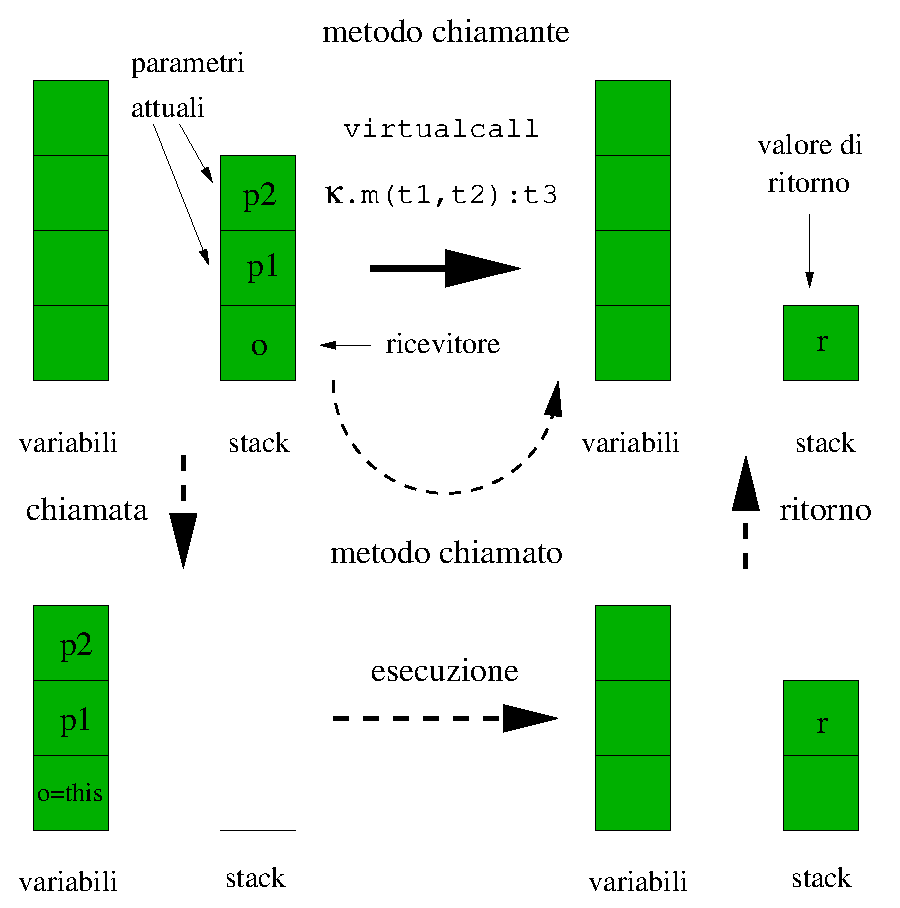
\epsfig{file = callercallee.eps, width = 12cm}
\end{center}
\caption{Il meccanismo di chiamata e ritorno da metodo.}
  \label{fig:callercallee}
\end{figure}

Il funzionamento complessivo del meccanismo di chiamata e ritorno da
costruttore o metodo \`e mostrato nella Figura~\ref{fig:callercallee}.
Il metodo chiamante prepara sullo stack degli operandi i parametri della
chiamata, incluso il ricevitore della chiamata,
indicato come $o$ in Figura~\ref{fig:callercallee}. Il metodo chiamato
\`e esplicito nel caso della chiamata a un costruttore, mentre per le chiamate
virtuali ai metodi
\`e identificato dinamicamente
a tempo di esecuzione sulla base della classe dell'oggetto a cui $o$ fa riferimento.
In entrambi i casi, esso
inizia la sua esecuzione in un frame di attivazione nuovo,
in cui le variabili locali contengono
i parametri della chiamata e lo stack degli operandi \`e vuoto.
Quando l'esecuzione del chiamato termina, se il metodo non ritorna
\texttt{void} allora la cima dello stack degli operandi del chiamato contiene
il valore di ritorno, $r$ in Figura~\ref{fig:callercallee}. La terminazione
del metodo riabilita il frame di attivazione del chiamato, in cui per\`o
lo stack degli operandi \`e stato privato dei parametri e arricchito con
il valore di ritorno $r$ del metodo.
%
\subsection{Le istruzioni di diramazione}\label{subsec:branching_bytecodes}
%
\begin{figure}[t]
\begin{center}
\begin{tabular}{|c|}
\hline\mbox{}\\
\mbox{}\\
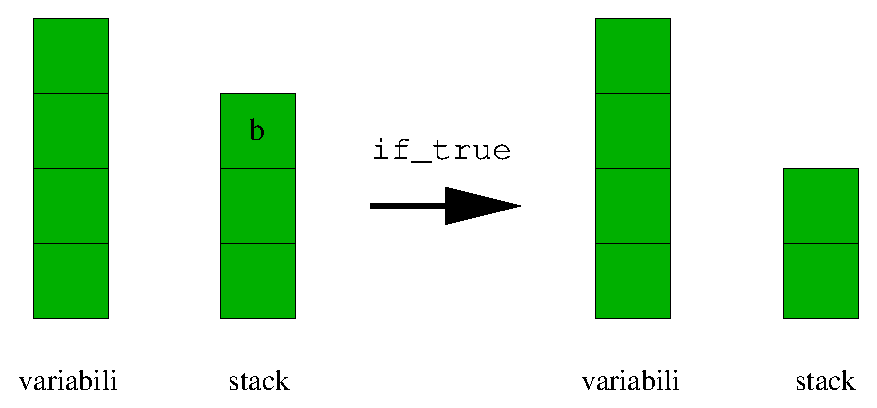
\epsfig{file = bytecodes/if_true.eps, width = 12cm}\\\hline
\mbox{}\\
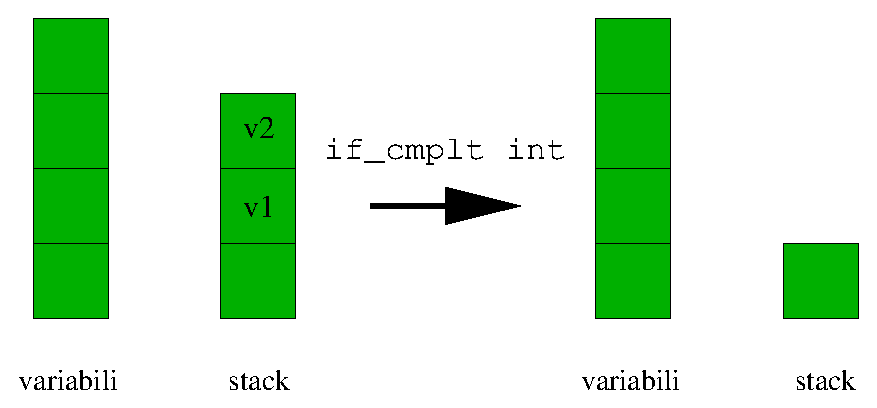
\epsfig{file = bytecodes/if_cmplt.eps, width = 12cm}\\\hline
\end{tabular}
\end{center}
\caption{Le istruzioni \texttt{if\_true} ed \texttt{if\_cmplt} del bytecode Kitten.}
  \label{fig:bytecodes9}
\end{figure}
%
Le istruzioni di diramazione
del bytecode Kitten sono sempre accoppiate all'inizio di due blocchi
di codice con lo stesso predecessore.
Esse indicano sotto quale condizione il controllo del
programma deve essere istradato verso uno dei due blocchi. Ne sono esempi le
istruzioni \texttt{if\_true} e \texttt{if\_false} in
Figura~\ref{fig:led_bytecode} e le istruzioni
\texttt{if\_cmplt int} e \texttt{if\_cmpge int} in
Figura~\ref{fig:fib_bytecode}.
Quando la condizione espressa dall'istruzione condizionale \`e vera, essa
viene eseguita, il che normalmente comporta l'eliminazione di alcuni
valori dallo stack degli operandi.

Vediamo in dettaglio l'insieme delle istruzioni di diramazione del
bytecode Kitten.
%
\begin{description}
\item[\underline{$\mathtt{if\_true}$}.]
  La condizione espressa da questa istruzione \`e che la cima dello stack degli
  operandi, che deve essere un booleano, sia il valore \texttt{true}.
  In tal caso il valore
  viene eliminato dallo stack (Figura~\ref{fig:bytecodes9}).
  Esiste anche l'istruzione simmetrica $\mathtt{if\_false}$.
\item[\underline{$\mathtt{if\_cmplt}\ t$}.]
  La condizione espressa da questa istruzione \`e che l'elemento che sta
  sotto la cima dello stack degli operandi sia minore dell'elemento che sta in
  cima allo stack. Entrambi gli elementi devono avere tipo $t$
  e vengono rimossi dallo
  stack (Figura~\ref{fig:bytecodes9}). Il tipo $t$ pu\`o essere \texttt{int}
  o \texttt{float}. Esistono anche le istruzioni $\mathtt{if\_cmple}$,
  $\mathtt{if\_cmpgt}$ ed $\mathtt{if\_cmpge}$. Esistono inoltre le
  istruzioni $\mathtt{if\_cmpeq}$ ed $\mathtt{if\_cmpne}$ la cui condizione,
  rispettivamente, \`e l'uguaglianza e la disuguaglianza dei due elementi
  in cima allo stack degli operandi. Queste ultime due istruzioni
  possono operare su tipi $t$ arbitrari, anche riferimento.
\end{description}
%
\subsection{L'implementazione del bytecode Kitten}
  \label{subsec:bytecode_implementation}
%
\begin{figure}[t]
\begin{center}
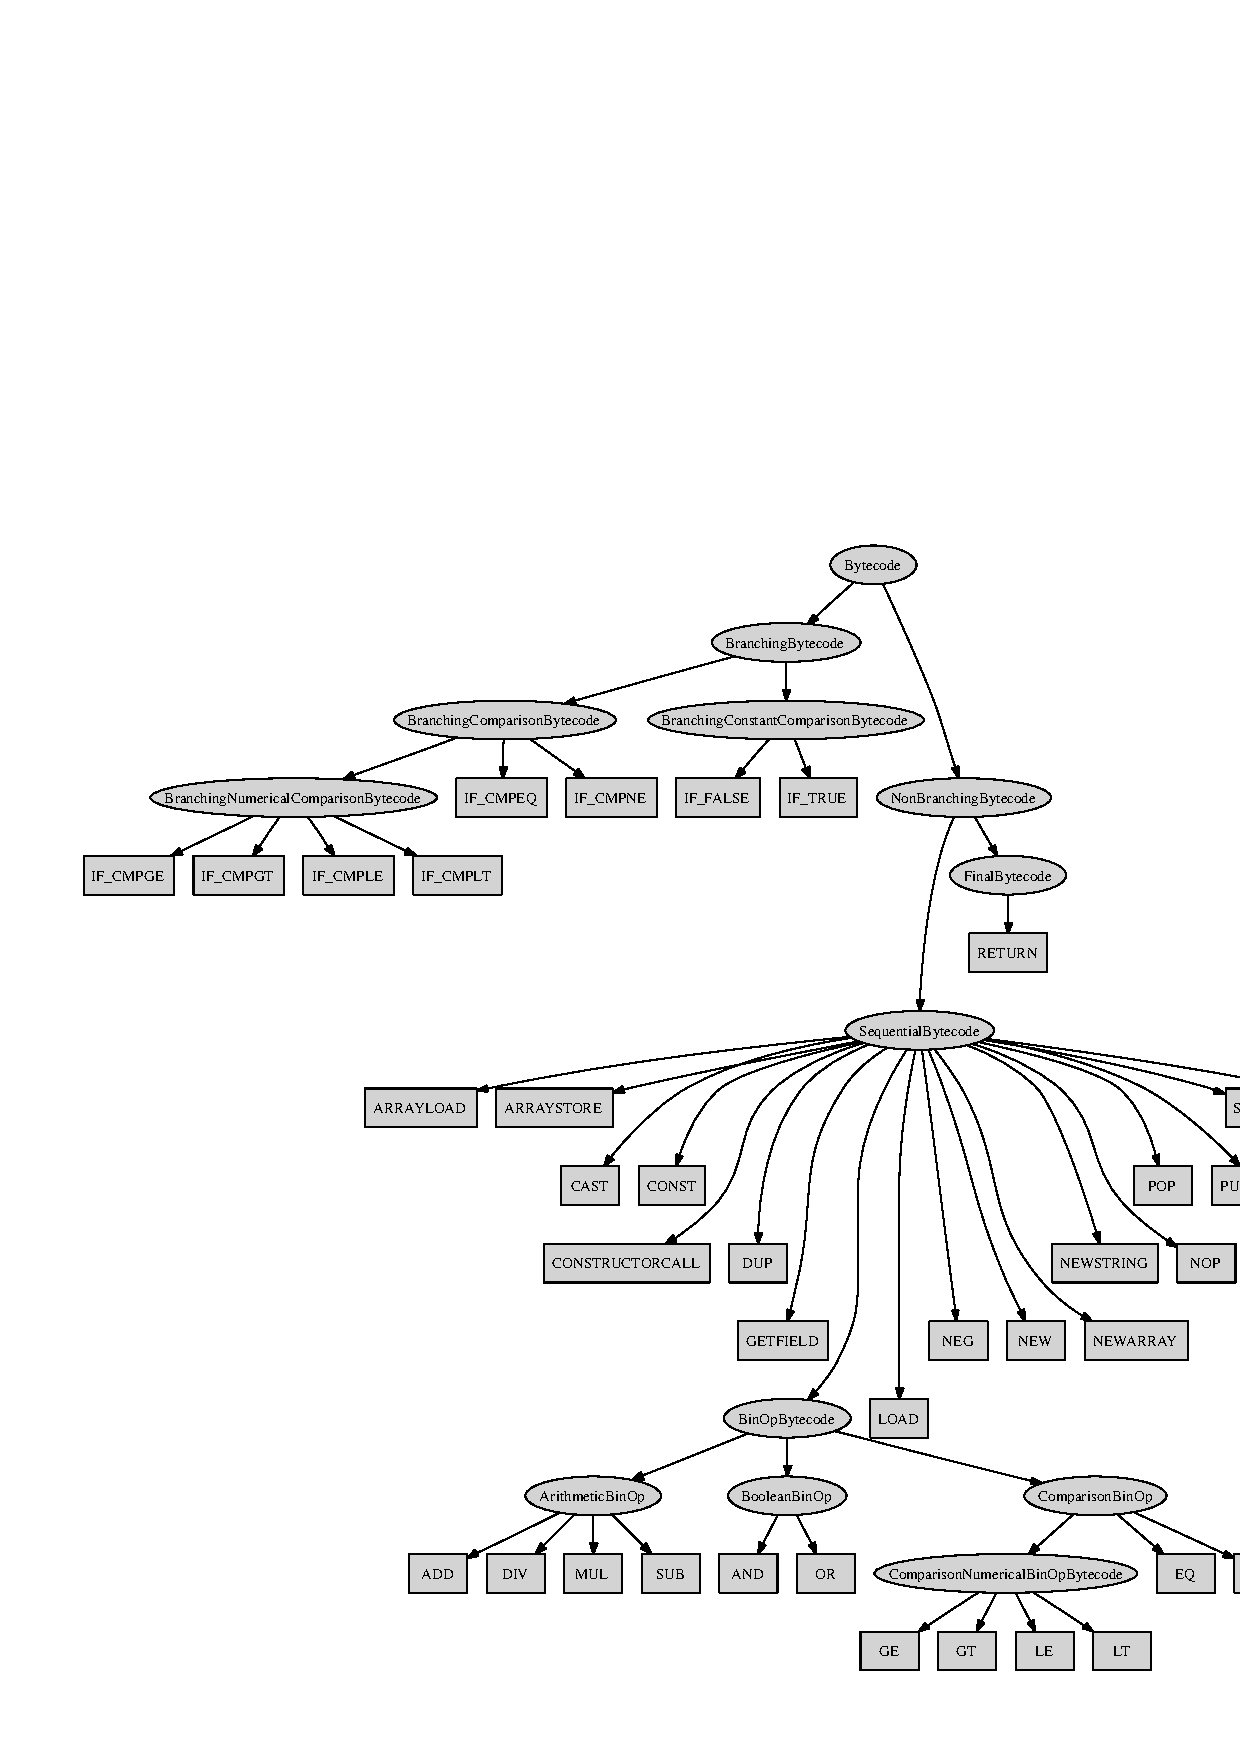
\includegraphics[width=15.5cm]{bytecodes_hierarchy.pdf}
\end{center}
\caption{La gerarchia delle classi del package \texttt{bytecode} che rappresentano le istruzioni del bytecode Kitten. Le classi ovali sono classi astratte, quelle rettangolari sono classi concrete.}
  \label{fig:bytecodes_hierarchy}
\end{figure}
%
Le istruzioni del bytecode Kitten che abbiamo descritto nelle sezioni
precedenti sono implementate nel package \texttt{bytecode}
come istanze della classe \texttt{bytecode/Bytecode.java}.
La gerarchia completa \e mostrata in Figura~\ref{fig:bytecodes_hierarchy}.
Le istruzioni vengono prima di tutto divise nelle due classi astratte
\texttt{NonBranchingBytecode} e \texttt{BranchingBytecode}.
La prima implementa le istruzioni sequenziali
delle Sezioni~\ref{subsec:sequential_bytecodes}
e~\ref{subsec:call_return}. La seconda implementa le istruzioni di
diramazione della Sezione~\ref{subsec:branching_bytecodes}.

La creazione di un bytecode avviene tramite il suo costruttore, che
richiede di specificare i tipi semantici su cui opera il bytecode.
Per esempio, un'istruzione \texttt{arrayload from array of int} si
crea con l'espressione Java
%
\begin{verbatim}
  new ARRAYLOAD(IntType.INSTANCE)
\end{verbatim}
%
La classe \texttt{bytecode/BytecodeList.java} implementa poi una lista
di bytecode che pu\`o essere inserita all'interno di un blocco di codice
(come in Figura~\ref{fig:fib_bytecode}). La struttura dati che implementa
tale blocco \e la classe \texttt{translate/CodeBlock.java} il cui costruttore
chiede di specificare la lista di bytecode contenuta nel blocco e la lista
dei successori del blocco (eventualmente vuota).

Un metodo importante della classe dei bytecode sequenziali \`e
\texttt{followedBy()}: esso richiede di specificare un blocco di codice
e restituisce un blocco ottenuto aggiungendo il bytecode in testa
al codice interno al blocco di codice. Per esempio, se il blocco di
codice $b$ contiene
%
\begin{verbatim}
  const 1
  return int
\end{verbatim}
%
allora \texttt{new IF\_TRUE().followedBy(b)} \e un blocco di codice che
contiene
%
\begin{verbatim}
  if_true
  const 1
  return int
\end{verbatim}
%
\section{La generazione del bytecode Kitten per le espressioni}
  \label{sec:expressions_bytecode_generation}
%
Mostriamo in questa sezione come tradurre
la sintassi astratta di un'espressione Kitten in del bytecode Kitten.

Abbiamo visto che un programma scritto in bytecode Kitten \`e un insieme
di blocchi all'interno dei quali si trova del codice,
come mostrato in Figura~\ref{fig:cycle_bytecode}.
Il bytecode che genereremo per le espressioni sar\`a in effetti molto
semplice, al punto che una sequenza di blocchi sar\`a
sempre sufficiente per tutte le espressioni. Si noti comunque che questa
propriet\`a
\e dovuta alla semplicit\`a delle espressioni del linguaggio Kitten e
che essa non sarebbe pi\`u vera se Kitten ammettesse ad esempio espressioni pi\`u
complesse, come l'espressione condizionale
$\mathit{exp}\ \mathtt{?}\ \mathit{exp}\ \mathtt{:}\ \mathit{exp}$
(si veda l'Esercizio~\ref{ex:conditional_expression_compilation}).

Ci sono tre contesti in cui un'espressione Kitten pu\`o trovarsi:
%
\begin{enumerate}
\item un contesto in cui di un'espressione serve il valore, come
      nel caso in cui essa occorre come lato destro di un assegnamento;
\item un contesto in cui di un'espressione serve sapere se \e vera o falsa
      per decidere come istradare l'esecuzione del programma, come nel
      caso in cui essa occorre come test di un condizionale. Ovviamente
      questo caso ha senso solo per le espressioni booleane;
\item un contesto in cui il valore di un'espressione deve essere modificato,
      come nel caso in cui essa occorre alla sinistra di un assegnamento.
      Ovviamente questo caso ha senso solo per i leftvalue.
\end{enumerate}
%
Compileremo un'espressione in tre modi diversi,
sulla base del contesto in cui essa occorre. Tali modi
sono detti rispettivamente
\emph{compilazione attiva}, \emph{compilazione condizionale} e
\emph{compilazione passiva} dell'espressione. Descriviamo adesso in
ordine questi tre tipi di compilazione delle espressioni.
%
\subsection{La compilazione attiva delle espressioni}
  \label{subsec:active_compilation}
%
Quando di un'espressione ci interessa il valore, allora l'esecuzione
del codice che vogliamo generare deve essere tale da:
%
\begin{enumerate}
\item lasciare intatti i valori iniziali sullo stack degli operandi;
\item aggiungere in cima allo stack degli operandi il valore dell'espressione.
\end{enumerate}
%
Questi due principi sono mostrati in Figura~\ref{fig:russian}. Il
vincolo 1 \`e importante poich\'e esso ci permette di valutare
in sequenza delle espressioni e ritrovarci alla fine i loro
valori sullo stack.
Questo \`e mostrato nella Figura~\ref{fig:russian_relevance},
che mostra l'esecuzione del codice che genereremo per l'and logico
di due espressioni $e_1$ ed $e_2$: prima generiamo del codice che
valuta $e_1$ e ne lascia il valore sullo stack, poi del codice che
valuta $e_2$ e ne lascia il valore sullo stack. Grazie al precedente vincolo
1, siamo certi che a questo punto il valore di $e_1$ \`e ancora nello stack,
sotto la cima. Possiamo quindi aggiungere un bytecode \texttt{and} per
ottenere il risultato cercato.

\begin{figure}[t]
\begin{center}
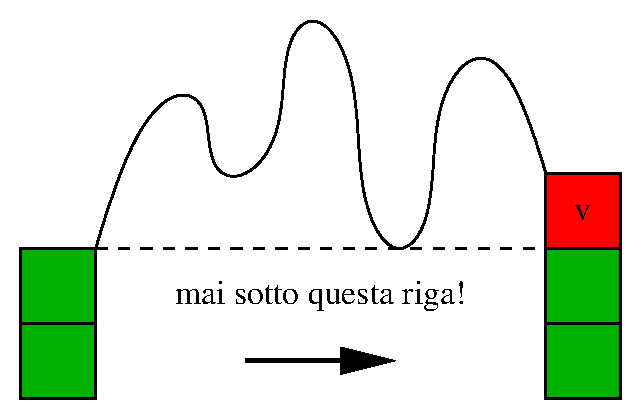
\epsfig{file = russe.eps, width = 8cm}
\end{center}
\caption{L'esecuzione del bytecode Kitten generato per un'espressione deve lasciare il valore dell'espressione sullo stack degli operandi e non deve modificare lo stack iniziale.}
  \label{fig:russian}
\end{figure}
%
\begin{figure}[t]
\begin{center}
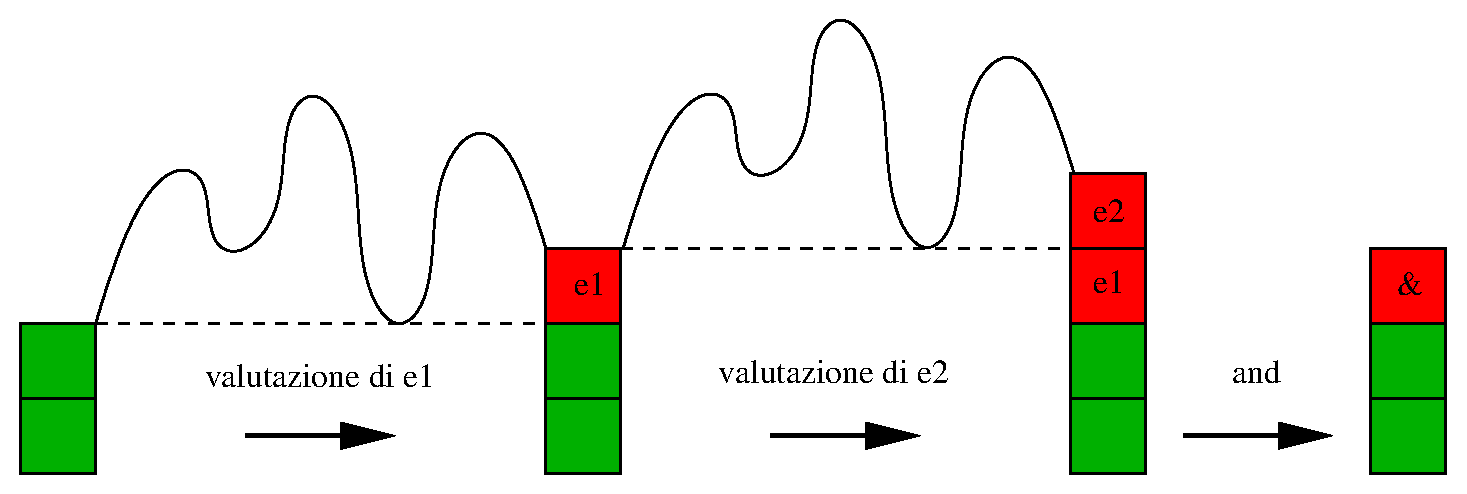
\epsfig{file = importanza.eps, width = 12cm}
\end{center}
\caption{L'esecuzione del bytecode Kitten per l'and logico di due espressioni $e_1$ ed $e_2$.}
  \label{fig:russian_relevance}
\end{figure}

Se $\beta$ \`e un blocco di codice, allora con la notazione
$\fbox{$\mathit{ins}$}\to\beta$
rappresentiamo un blocco di codice
al cui interno si trova l'istruzione (o le istruzioni) $\mathit{ins}$
e che ha $\beta$ come successore.
La Figura~\ref{fig:expressions_generation} usa tale notazione per
definire le regole per la
generazione del codice per le espressioni Kitten. Esse sono formalizzate
tramite una funzione $\gen{\_}$ che associa alla sintassi astratta
delle espressioni il bytecode Kitten che ne calcola il valore e lo lascia
in cima allo stack degli operandi.
Tale funzione richiede in primo luogo di specificare l'espressione $e$
di cui si vuole generare il bytecode. La notazione $\gen{e}$ \`e
per\`o ancora una funzione da $\mathtt{translate.CodeBlock}$ in
$\mathtt{translate.CodeBlock}$, \cioe la classe usata per
rappresentare un blocco di bytecode
(Sezione~\ref{subsec:bytecode_implementation}). In particolare, quello che
occorre ancora specificare \`e il bytecode $\beta$
che deve essere eseguito \emph{dopo} la valutazione di $e$.
Il bytecode $\gen{e}(\beta)$ sar\`a quindi il bytecode che \emph{prima}
valuta l'espressione $e$, lasciandone il valore sullo stack degli operandi,
e \emph{dopo} esegue il codice $\beta$. Per esempio, la
Figura~\ref{fig:expressions_generation} implica che
\[
  \gen{\mathtt{IntLiteral(3)}}(\fbox{$\mathtt{return\ int}$})
    =\fbox{$\mathtt{const\ 3}$}\to\fbox{$\mathtt{return\ int}$}
\]

Questo modo di generare il codice
si chiama \emph{compilazione con continuazioni} e $\beta$ \`e detta
la \emph{continuazione} della compilazione di $e$. La compilazione per
continuazioni \`e molto elegante \poiche permette di semplificare la fusione
fra il codice generato per due parti sequenziali di un programma.
%
\begin{figure}[t]
{\scriptsize
\begin{align*}
  \gen{\_}:\mathtt{absyn.Expression}&\mapsto(\mathtt{translate.CodeBlock}\mapsto\mathtt{translate.CodeBlock})\\
  \mbox{}\\
  \gen{\mathtt{Variable(\mathit{name})}}(\beta)&=\fbox{\texttt{load $\mathit{num}$ of type $\tau$}}\to\beta\\
  \text{dove $\mathit{num}$ \`e il numero}&\text{ progressivo della variabile \textit{name} nel metodo corrente}\\
  \gen{\mathtt{FieldAccess(\mathit{receiver},\mathit{name})}}(\beta)&=
    \gen{\mathit{receiver}}\left(\fbox{\texttt{getfield $\mathit{field}$}}
    \to\beta\right)\\
  \text{dove $\mathit{field}$ \`e il campo}&\text{ identificato
    dall'analisi semantica (Figura~\ref{fig:analysis_expressions1})}\\
  \gen{\mathtt{ArrayAccess(\mathit{array},\mathit{index})}}(\beta)&=
    \gen{\mathit{array}}\left(\gen{\mathit{index}}\left(
    \fbox{$\mathtt{arrayload\ from\ array\ of\ }\tau$}\to\beta\right)\right)\\
  \gen{\mathtt{True()}}(\beta)=\fbox{$\mathtt{const\ true}$}\to\beta&\qquad
  \gen{\mathtt{False()}}(\beta)=\fbox{$\mathtt{const\ false}$}\to\beta\\
  \gen{\mathtt{IntLiteral(\mathit{value})}}(\beta)
    &=\gen{\mathtt{FloatLiteral(\mathit{value})}}(\beta)
    =\fbox{$\mathtt{const}\ \mathit{value}$}\to\beta\\
  \gen{\mathtt{String(\mathit{value})}}(\beta)
    =\fbox{$\mathtt{newstring}\ \mathit{value}$}\to\beta&\qquad
    \gen{\mathtt{Nil()}}(\beta)=\fbox{$\mathtt{const\ nil}$}\to\beta\\
  \gen{\mathtt{NewObject(\mathit{className},\mathit{actuals})}}(\beta)
    &=\fbox{$\begin{array}{l}
      \mathtt{new}\ \kappa\\
      \mathtt{dup}\ \kappa
    \end{array}$}\to
   \gentwo{\vec{t}}{\mathit{actuals}}
   \left(\fbox{$\mathtt{constructorcall}\ \mathit{con}$}\to\beta\right)\\
  \text{dove $\mathit{con}=\kappa(\vec{t})\mathtt{:void}$ \e il}&
  \text{ costruttore identificato dall'analisi semantica
        (Figura~\ref{fig:analysis_expressions2})}\\
  \gen{\mathtt{NewArray(\mathit{elementsType},\mathit{size})}}(\beta)
    &=\gen{\mathit{size}}
    \left(\fbox{$\mathtt{newarray\ of\ }\tau\mathtt{.getElementsType()}$}
    \to\beta\right)\\
  \gen{\mathtt{MethodCallExpression(\mathit{receiver},\mathit{name},
    \mathit{actuals})}}&=\gen{\mathit{receiver}}\left(
    \gentwo{\vec{t}}{\mathit{actuals}}
    \left(\fbox{$\mathtt{virtualcall}\ \mathit{method}$}
    \to\beta\right)\right)\\
  \text{dove $\mathit{method}=\kappa.\mathtt{m}(\vec{t}):t'$
        \`e il}&
  \text{ metodo identificato dall'analisi semantica
        (Figura~\ref{fig:analysis_expressions2})}\\
  \gen{\mathtt{Not(\mathit{expression})}}(\beta)=
    \gen{\mathtt{Minus(\mathit{expression})}}(\beta)&=
    \gen{\mathit{expression}}\left(
    \fbox{$\mathtt{neg\ }\tau$}\to\beta\right)\\
  \gen{\mathtt{Cast(\mathit{\mathit{type},\mathit{expression}})}}(\beta)=
      \gen{\mathit{expression}}&
        \left(\fbox{$\mathtt{cast\ from\ }\tau'\mathtt{\ into\ }\tau$}
        \to\beta\right)
  \quad\text{con $\tau'$ \e tipo statico di }\mathit{expression}\\
  \gen{\mathtt{And(\mathit{left},\mathit{right})}}(\beta)&=
    \gen{\mathit{left}}\left(
      \gen{\mathit{right}}\left(\fbox{$\mathtt{and}$}\to\beta\right)\right)\\
  \gen{\mathtt{Addition(\mathit{left},\mathit{right})}}(\beta)&=
    \gentwo{\tau}{\mathit{left}}\left(
      \gentwo{\tau}{\mathit{right}}\left(\fbox{$\mathtt{add}\ \tau$}
      \to\beta\right)\right)\\
  \gen{\mathtt{LessThanOrEqual(\mathit{left},\mathit{right})}}(\beta)=
    \gentwo{\ell}{\mathit{left}}\Big(
      \gentwo{\ell}{\mathit{right}}&\left(\fbox{$\mathtt{le}\ \ell$}
      \to\beta\right)\Big)\quad
  \text{con $\ell$ minimo supertipo comune fra il tipo statico di
    $\mathit{left}$ e di $\mathit{right}$}
\end{align*}
}
\caption{La funzione $\gen{\_}$ che genera il bytecode Kitten che valuta le espressioni. Il tipo $\tau$ \`e il tipo statico assegnato all'espressione durante la sua analisi semantica.}
  \label{fig:expressions_generation}
\end{figure}

La Figura~\ref{fig:expressions_generation} usa la funzione
$\gentwo{\tau}{e}$ che rispetto a $\gen{e}$ effettua in pi\`u,
se necessario, la promozione a $\tau$ del valore dell'espressione $e$.
In Kitten essa \e utile ogni qual volta si usa un valore intero
in un punto in cui si richiedeva un valore in virgola mobile come
per esempio nell'espressione $\mathtt{3\ +\ 4.5}$, in cui occorre convertire
il valore intero $3$ in un $\mathtt{float}$ prima di sommarlo con
il valore $4.5$. Quando potrebbe essere necessaria una promozione di tipo
del valore di un'espressione, la Figura~\ref{fig:expressions_generation}
compila l'espressione tramite $\gentwo{\tau}{\_}$ piuttosto
che tramite $\gen{\_}$.
Lo stesso fenomeno lo incontreremo fra poco con i comandi,
in un assegnamento del tipo:
%
\begin{verbatim}
  float f := 13
\end{verbatim}
%
dove l'intero $13$ deve essere convertito in \texttt{float} prima
dell'assegnamento.
Tale funzione di conversione \`e definita a partire da $\gen{e}$:
\begin{equation}\label{eq:gentwo}
  \gentwo{\tau}{e}(\beta)=\begin{cases}
    \gen{e}(\fbox{$\mathtt{cast\ from\ int\ into\ float}$}\to\beta) &
      \text{se $\tau$ \`e $\mathtt{float}$ ed
            $e$ ha tipo statico $\mathtt{int}$}\\
    \gen{e}(\beta) & \text{altrimenti.}
  \end{cases}
\end{equation}
Per esempio,
%
\begin{align*}
  \gentwo{\mathtt{int}}{\mathtt{IntLiteral(3)}}(\fbox{$\mathtt{return\ int}$})
    &=\gen{\mathtt{IntLiteral(3)}}(\fbox{$\mathtt{return\ int}$})\\
  &=\fbox{$\mathtt{const\ 3}$}\to\fbox{$\mathtt{return\ int}$}
\end{align*}
%
mentre
%
\begin{align*}
  &\quad\gentwo{\mathtt{float}}{\mathtt{IntLiteral(3)}}
    (\fbox{$\mathtt{return\ float}$})\\
  &=\gen{\mathtt{IntLiteral(3)}}(\fbox{$\mathtt{cast\ from\ int\ into\ float}$}
    \to\fbox{$\mathtt{return\ float}$})\\
  &=\fbox{$\mathtt{const\ 3}$}\to\fbox{$\mathtt{cast\ from\ int\ into\ float}$}
    \to\fbox{$\mathtt{return\ float}$.}
\end{align*}
%
L'esempio precedente sarebbe quello di un'istruzione
$\mathtt{return\ 3}$ che occorre all'interno di un metodo il cui
tipo di ritorno \`e $\mathtt{float}$.
La notazione $\gentwo{\tau}{\_}$ viene infine
estesa a sequenze di espressioni e di tipi (di uguale lunghezza),
ottenendo la notazione $\gentwo{\vec{t}}{\_}$, definita come segue:
%
\begin{align*}
  \gentwo{\epsilon}{\mathtt{null}}(\beta)&=\beta\\
  \gentwo{\tau::\vec{t}}{\mathtt{ExpressionSeq(\mathit{head},
    \mathit{tail})}}(\beta)&=\gentwo{\tau}{\mathit{head}}(\gentwo{\vec{t}}
    {\mathit{tail}}(\beta))~.
\end{align*}
%
Per esempio:
%
{\small
\begin{align*}
  &\hspace*{-5ex}\gentwotwo{\mathtt{float}::\mathtt{float}}
    {\begin{array}{c}
     \mathtt{ExpressionSeq(FloatLiteral(3.4),}\\
     \mathtt{ExpressionSeq(IntLiteral(4),null))}
     \end{array}}
    (\fbox{$\mathtt{add\ float}$})\\
  &=\gentwo{\mathtt{float}}{\mathtt{FloatLiteral(3.4)}}
    (\gentwo{\mathtt{float}}{\mathtt{IntLiteral(4)}}
    (\fbox{$\mathtt{add\ float}$}))\\
  &=\gentwo{\mathtt{float}}{\mathtt{FloatLiteral(3.4)}}
    (\fbox{$\mathtt{const\ 4}$}\to\fbox{$\mathtt{cast\ from\ int\ to\ float}$}
    \to\fbox{$\mathtt{add\ float}$})\\
  &=\fbox{$\mathtt{const\ 3.4}$}
    \to\fbox{$\mathtt{const\ 4}$}\to\fbox{$\mathtt{cast\ from\ int\ to \ float}$}
    \to\fbox{$\mathtt{add\ float}$.}
\end{align*}}

Commentiamo adesso le regole di generazione del bytecode Kitten in
Figura~\ref{fig:expressions_generation}.
%
\begin{description}
\item[\underline{$\mathtt{Variable(\mathit{name})}$}.]
  Per caricare sullo stack il valore di una variabile locale, usiamo
  il bytecode \texttt{load} della Figura~\ref{fig:bytecodes2}.
  Il numero della variabile locale \`e gi\`a stato determinato in
  fase di analisi semantica e accessibile tramite il type-checker usato
  per l'analisi, insieme al tipo della variabile
  (Figura~\ref{fig:semantical.TypeChecker}).
\item[\underline{$\mathtt{FieldAccess(\mathit{receiver},\mathit{name})}$}.]
  Per accedere a un campo dell'oggetto $o$
  contenuto in $\mathit{receiver}$,
  generiamo inizialmente il bytecode che lascia sullo stack degli operandi
  il riferimento ad $o$. Questo \`e ottenuto richiamando ricorsivamente
  la generazione del bytecode per $\mathit{receiver}$. Come continuazione,
  gli passiamo un blocco che contiene un bytecode
  $\mathtt{getfield}$ (Figura~\ref{fig:bytecodes6})
  e che \`e legato alla continuazione $\beta$.
  L'effetto globale \`e quindi quello di valutare $\mathit{receiver}$,
  leggere il valore del campo di nome $\mathit{name}$ e quindi continuare
  con la continuazione $\beta$. Si noti che il campo da leggere \`e gi\`a
  stato identificato in fase di analisi semantica ($\mathit{field}$ in
  Figura~\ref{fig:analysis_expressions1}).
\item[\underline{$\mathtt{ArrayAccess(\mathit{array},\mathit{index})}$}.]
  Leggere un elemento di un array richiede in primo luogo di
  valutare l'espressione che contiene il riferimento all'array. Questo \`e
  ottenuto compilando ricorsivamente $\mathit{array}$. Come continuazione
  gli diamo la compilazione di $\mathit{index}$, seguita dal bytecode
  $\mathtt{arrayload}$ e dalla
  continuazione $\beta$. Si noti che il tipo statico $\tau$
  dell'array \`e gi\`a stato calcolato in fase di analisi semantica.
  Il bytecode $\mathtt{arrayload}$ consumer\`a dallo stack
  il riferimento all'array e l'indice da cui leggere e li sostituir\`a
  con il valore dell'elemento letto (Figura~\ref{fig:bytecodes7}).
\item[\underline{$\mathtt{True()}$},
      \underline{$\mathtt{False()}$},
      \underline{$\mathtt{IntLiteral(\mathit{value})}$},
      \underline{$\mathtt{FloatLiteral(\mathit{value})}$},
      \underline{$\mathtt{String(\mathit{value})}$},
      \underline{$\mathtt{Nil()}$}.]
  Dal mo-\linebreak
  mento che queste
  classi di sintassi astratta rappresentano delle costanti,
  usiamo il bytecode $\mathtt{const}$ della Figura~\ref{fig:bytecodes2}
  e $\mathtt{newstring}$ della Figura~\ref{fig:bytecodes4} per caricare tali
  costanti in cima allo stack.
\item[\underline{$\mathtt{NewObject(\mathit{className,\mathit{actuals}})}$}.]
  Questo nodo di sintassi astratta per la creazione di un oggetto di classe
  $\mathit{className}$ \e stato annotato durante l'analisi semantica con
  il costruttore $\mathit{con}=
  \kappa(\vec{t})\mathtt{:void}$ della classe $\kappa$ che \`e
  il corrispondente semantico di $\mathit{className}$. Tale costruttore
  \e il \piu
  specifico fra quelli che possono essere chiamati da questa espressione
  sulla base del tipo
  statico dei parametri attuali (Figura~\ref{fig:analysis_expressions2}).
  Il codice che generiamo inizia con un bytecode $\mathtt{new}\ \kappa$ che
  crea un nuovo oggetto $o$ di classe $\kappa$ e ne pone in cima allo stack
  un riferimento (Figura~\ref{fig:bytecodes4}). Tale riferimento
  viene quindi duplicato dal bytecode $\mathtt{dup}\ \kappa$
  (Figura~\ref{fig:bytecodes1}).
  Segue la compilazione dei parametri attuali del costruttore.
  A questo punto sullo stack troviamo due copie di un riferimento
  ad $o$ sormontate dai valori dei parametri
  attuali. Con il bytecode \texttt{constructorcall} otteniamo quindi di
  chiamare il costruttore legando $\mathtt{this}$ ad $o$ e i parametri
  attuali ai parametri formali (Figura~\ref{fig:bytecodes8}).
  Per esempio, la compilazione di
  \begin{multline*}
    \mathtt{NewObject(\mathit{className},}\\
    \mathtt{ExpressionSeq(IntLiteral(3),ExpressionSeq(IntLiteral(4),null)))}
  \end{multline*}
  \e
  \[\begin{array}{l}
    \mathtt{new}\ \kappa\\
    \mathtt{dup}\ \kappa\\
    \mathtt{const\ 3}\\
    \mathtt{const\ 4}\\
    \mathtt{constructorcall\ \mathit{con}}
  \end{array}\]
  seguita dalla continuazione $\beta$ (nell'ipotesi che non serva promozione
  di tipo nel passaggio dei parametri interi al costruttore).
  Dalla Figura~\ref{fig:bytecodes8} sappiamo che
  il bytecode \texttt{constructorcall}
  rimuove dallo stack degli operandi sia i parametri attuali che $o$.
  Questo \`e il motivo per cui usiamo il bytecode $\mathtt{dup}$:
  senza di esso il riferimento ad $o$ andrebbe perso dallo stack
  e avremmo ottenuto di inizializzare un oggetto che subito dopo
  diventava irraggiungibile.
\item[\underline{$\mathtt{NewArray(\mathit{elementsType},\mathit{size})}$}.]
  Il bytecode generato per la creazione di un array inizia con
  la compilazione dell'espressione $\mathit{size}$ che lascia in cima allo
  stack la dimensione richiesta per l'array.
  Basta quindi proseguire il codice con un bytecode $\mathtt{newarray}$ che
  consuma tale dimensione e la sostituisce con un riferimento a un nuovo
  array (Figura~\ref{fig:bytecodes5}). Segue la continuazione $\beta$.
  Si ricordi che il tipo statico $\tau$ di questa espressione \`e il tipo
  dell'array che stiamo creando (Figura~\ref{fig:analysis_expressions2}).
\item[\underline{$\mathtt{MethodCallExpression(\mathit{receiver},\mathit{name},
  \mathit{actuals})}$}.]
  L'invocazione di un metodo \`e compilata in modo molto simile all'invocazione
  di un costruttore per un nodo $\mathtt{NewObject}$ di sintassi astratta
  (si veda sopra). La differenza \`e che si usa il bytecode
  $\mathtt{virtualcall}$ invece di $\mathtt{constructorcall}$
  (Figura~\ref{fig:bytecodes8}). Inoltre il riferimento all'oggetto
  ricevitore della chiamata \`e il valore lasciato sullo stack dal
  bytecode generato per $\mathit{receiver}$, piuttosto che un nuovo oggetto
  come per $\mathtt{NewObject}$. Si ricordi che l'analisi semantica ha
  garantito che il metodo invocato ha un tipo di ritorno diverso da
  $\mathtt{void}$ (Figura~\ref{fig:analysis_expressions2}). Siamo quindi
  sicuri che il bytecode $\mathtt{virtualcall}$ lascia sullo stack un
  valore di ritorno (Figura~\ref{fig:bytecodes8}), che \`e il valore di
  questa espressione d'invocazione di un metodo.
\item[\underline{$\mathtt{Not(\mathit{expression})}$} e
  \underline{$\mathtt{Minus(\mathit{expression})}$}.]
  Entrambe queste espressioni sono compilate in del bytecode che
  inizia con la compilazione ricorsiva di $\mathit{expression}$ e continua
  con il bytecode $\mathtt{neg}$ (Figura~\ref{fig:bytecodes3})
  e con la continuazione $\beta$. Si noti comunque che il tipo $\tau$
  su cui opera $\mathtt{neg}$ \`e diverso: esso \`e $\mathtt{boolean}$
  per $\mathtt{Not}$ ed \`e $\mathtt{int}$ oppure $\mathtt{float}$ per
  $\mathtt{Minus}$ (Figura~\ref{fig:analysis_expressions2}).
\item[\underline{$\mathtt{Cast(\mathit{type},\mathit{expression})}$}.]
  La compilazione di un cast verso il basso \`e essenzialmente la compilazione
  dell'espressione di cui si sta facendo il cast, seguita dalla continuazione
  $\beta$. In \piu inseriamo un bytecode $\mathtt{cast}$
  che effettua il cast o la conversione di tipo da
  $\mathtt{float}$ ad $\mathtt{int}$ (Figura~\ref{fig:bytecodes5})
  nel caso in cui il cast sia in effetti
  una richiesta di arrotondamento di un valore a virgola mobile
  ($\mathtt{3.14\ as\ int}$). Si noti la differenza fra queste due
  situazioni: la conversione da $\mathtt{float}$ a $\mathtt{int}$
  modifica la rappresentazione binaria del valore in cima allo stack ma
  non pu\`o mai fallire (sappiamo con certezza che in cima allo stack
  c'\`e un $\mathtt{float}$). La verifica di tipo non effettua invece
  alcuna modifica sul valore in cima allo stack, ma pu\`o fallire
  bloccando l'esecuzione del programma.
\item[\underline{$\mathtt{BinOp(\mathit{left},\mathit{right})}$}.]
  La compilazione di un'operazione binaria \`e il codice formato
  dalla compilazione di $\mathit{left}$ seguita dalla compilazione
  di $\mathit{right}$ seguita da un bytecode che implementa
  l'operazione binaria opportuna e infine dalla continuazione $\beta$.
  Gli esempi mostrati in Figura~\ref{fig:expressions_generation}
  presentano tutte le tipologie di espressioni binarie.
  Quelle logiche usano un bytecode $\mathtt{and}$ od $\mathtt{or}$ per
  il quale non serve specificare il tipo degli operandi (\`e sempre
  $\mathtt{boolean}$). Quelle aritmetiche possono invece
  operare sia su $\mathtt{int}$ che su $\mathtt{float}$ e i loro
  operandi potrebbero richiedere una promozione di tipo, per cui usiamo
  per essi $\gentwo{\tau}{\_}$ piuttosto che $\gen{\_}$. Le operazioni
  binarie di confronto possono operare su tipo arbitrari e possono
  anch'esse richiedere una conversione di tipo per gli operandi.
\end{description}

Consideriamo adesso l'implementazione delle regole di compilazione
in Figura~\ref{fig:expressions_generation}. Un blocco di codice
lo implementiamo come un oggetto di classe
$\mathtt{translate.CodeBlock}$ contenente una lista
di bytecode Kitten ed eventualmente legato ad altri blocchi successori.
L'implementazione della funzione $\gamma$ \e
ottenuta tramite i seguenti due metodi aggiunti
ad $\mathtt{absyn/Expression.java}$:
%
\begin{verbatim}
  protected abstract CodeBlock translate(CodeBlock continuation);

  public final CodeBlock translateAs(Type type, CodeBlock continuation) {
    if (staticType == IntType.INSTANCE && type == FloatType.INSTANCE)
      continuation = new CAST(IntType.INSTANCE, FloatType.INSTANCE)
                       .followedBy(continuation);
    else
      return translate(continuation);
  }
\end{verbatim}
%
Il primo implementa $\gen{\_}$ ed
\`e lasciato \texttt{abstract}. Esso verr\`a istanziato nelle
sottoclassi di $\mathtt{absyn.Expression}$
con l'implementazione delle regole in
Figura~\ref{fig:expressions_generation}. Il secondo implementa la funzione
$\gentwo{\tau}{\_}$ dell'Equazione~\ref{eq:gentwo}. Si noti l'uso di
\texttt{followedBy()} per aggiungere un bytecode in cima a un blocco di codice.

Mostriamo alcuni esempi di istanziazione del metodo
$\mathtt{translate()}$. In \texttt{absyn/True.java} definiamo
%
\begin{verbatim}
  public final CodeBlock translate(CodeBlock continuation) {
    return new CONST(true).followedBy(continuation);
  }
\end{verbatim}
%
che rispecchia fedelmente quanto riportato in
Figura~\ref{fig:expressions_generation}.

In \texttt{absyn/Variable.java} defininiamo
%
\begin{verbatim}
  public CodeBlock translate(CodeBlock continuation) {
    return new LOAD(getVarNum(), getStaticType()).followedBy(continuation);
  }
\end{verbatim}
%
Il numero della variabile era stato annotato in fase di analisi semantica
(Sezione~\ref{subsec:analysis_expressions_implementation}).
Utilizziamo anche il tipo
$\tau$ annotato per questa espressione, accessibile tramite
\texttt{getStaticType()}. Ancora una volta, questa implementazione
riflette la definizione in Figura~\ref{fig:expressions_generation}.

Dentro \texttt{absyn/BinOp.java} definiamo
%
\begin{verbatim}
  public final CodeBlock translate(CodeBlock continuation) {
    Type ell = getLeft().getStaticType()
      .leastCommonSupertype(getRight().getStaticType());
    return getLeft().translateAs
      (ell, getRight().translateAs
       (ell, operator(ell).followedBy(continuation)));
  }

  protected abstract BinOpBytecode operator(Type type);
\end{verbatim}
%
L'idea \`e di calcolare il minimo sovratipo comune $\ell$
fra i tipi statici dei due operandi, compilarli entrambi con
$\gentwo{\mathit{\ell}}{\_}$ e farli quindi seguire da un bytecode binario
specifico all'operazione binaria che si sta compilando. Tale bytecode
\`e fornito dal metodo ausiliario \texttt{operator()} che \`e per esempio
definito dentro $\mathtt{absyn/Addition.java}$ come
%
\begin{verbatim}
  protected BinOpBytecode operator(Type type) {
    return new ADD((NumericalType) type);
  }
\end{verbatim}
%
Si noti che questo modo di procedere generalizza le tre ultime regole
in Figura~\ref{fig:expressions_generation}.
%
\subsection{La compilazione condizionale delle espressioni booleane}
  \label{subsec:conditional_generation}
%
Abbiamo descritto come un'espressione venga tradotta in del bytecode
Kitten che ne calcola il valore e lo lascia in cima allo stack degli
operandi. Tale codice \e adeguato se quello a cui
siamo interessati \`e il valore dell'espressione. Per esempio, di un parametro
passato a un metodo abbiamo bisogno del valore, \cosi come del lato destro
di un assegnamento.
Ci sono casi per\`o in cui quello che ci interessa \`e di istradare
l'esecuzione di un programma in due direzioni diverse sulla base
del valore di un'espressione booleana. Per esempio, nel comando
$\mathtt{if\ (\mathit{exp})\ then\ \mathit{com}_{\rm 1}
\ else\ \mathit{com}_{\rm 2}}$
siamo interessati a eseguire $\mathit{com}_1$ se il valore
di $\mathit{exp}$ \`e $\mathit{true}$ e a eseguire $\mathit{com}_2$
se tale valore \`e invece $\mathit{false}$. Occorre quindi definire
un altro modo di generare il bytecode per le espressioni,
alternativo a quello della
Figura~\ref{fig:expressions_generation} e che chiameremo
\emph{compilazione condizionale} delle espressioni. Va comunque detto che
ricicleremo in larghissima misura le definizioni in tale figura. Va ricordato
inoltre che
la compilazione condizionale ha senso solo per le espressioni che hanno
tipo \texttt{boolean},
dal momento che l'analisi semantica ci garantisce che esse sono le uniche
che possono essere usate nei test dei condizionali e dei cicli
(Figura~\ref{fig:analysis_expressions2}).

Definiamo quindi una funzione
%
\begin{multline*}
  \gentest{\_}{}{}:\mathtt{absyn.Expression}\to
    \mathtt{translate.CodeBlock}\\
  \mapsto\mathtt{translate.CodeBlock}
    \mapsto\mathtt{translate.CodeBlock}
\end{multline*}
%
che compila un'espressione in maniera condizionale.
In particolare, $\gentest{\mathit{exp}}(\beta_\mathit{true})
(\beta_\mathit{false})$ \`e la
compilazione condizionale dell'espressione $\mathit{exp}$:
se l'espressione contiene $\mathit{true}$ l'esecuzione
viene istradata verso la continuazione $\beta_\mathit{true}$;
altrimenti verso la continuazione $\beta_\mathit{false}$.
La sua definizione sfrutta quella in Figura~\ref{fig:expressions_generation}:
%
\begin{equation}\label{eq:conditional_compilation}
  \gentest{\mathit{exp}}(\beta_{\mathit{true}})(\beta_\mathit{false})=
    \gen{\mathit{exp}}\left(
      \fbox{$\mathtt{nop}$}\,\,\langle
    \begin{array}{l}
        \fbox{$\mathtt{if\_true}$}\to\beta_{\mathit{true}}\\
        \fbox{$\mathtt{if\_false}$}\to\beta_\mathit{false}
    \end{array}
    \right)
\end{equation}
%
Per esempio, supponendo che la variabile $\mathtt{i}$ sia allocata nella
variabile locale numero $1$ e che abbia tipo \texttt{int},
allora la compilazione condizionale di \texttt{i < 5} \`e
%
\[
  \fbox{$
  \begin{array}{l}
    \mathtt{load\ 1\ of\ type\ int}\\
    \mathtt{const\ 5}\\
    \mathtt{lt\ int}
  \end{array}
  $}\to
  \fbox{$\mathtt{nop}$}\,\,\langle
    \begin{array}{l}
        \fbox{$\mathtt{if\_true}$}\to\beta_{\mathit{true}}\\
        \fbox{$\mathtt{if\_false}$}\to\beta_\mathit{false}
    \end{array}
\]

La funzione $\gentest{\_}$ \`e implementata
aggiungendo ad \texttt{absyn.Expression} il metodo:
%
\begin{verbatim}
  public CodeBlock translateAsTest(CodeBlock yes, CodeBlock no) {
    return translate(new CodeBlock(new IF_TRUE(), yes, no));
  }
\end{verbatim}
%
Il costruttore utilizzato per questo \texttt{CodeBlock} costruisce
un blocco con codice \texttt{nop} e legato alle continuazioni
\texttt{yes} e \texttt{no} tramite, rispettivamente, il bytecode condizionale
\texttt{if\_true} e il suo opposto.

La definizione di $\gentest{\_}$ che abbiamo appena visto funziona per
qualsiasi espressione condizionale. Genera per\`o del codice
particolarmente ridondante. Per esempio, la compilazione condizionale
di \texttt{i < 5} che abbiamo ottenuto sopra \`e molto meno ottimizzata
di quella in Figura~\ref{fig:cycle_bytecode}, che non usa n\'e l'istruzione
\texttt{nop} n\'e la \texttt{lt int} e usa invece i bytecode condizionali
\texttt{if\_cmplt int} ed \texttt{if\_cmpge int} al posto di
\texttt{if\_true} ed \texttt{if\_false}. Il problema della \texttt{nop}
non deve preoccuparci: una volta
generato il bytecode per una classe Kitten, elimineremo
tutte le \texttt{nop} dal codice. Per usare invece dei bytecode condizionali
specializzati, possiamo aggiungere delle definizioni specifiche
per la funzione $\gentest{\_}$, che ridefiniscono la precedente definizione
generale su dei casi particolari molto frequenti. Per esempio definiamo
%
\[
  \gentest{\mathtt{LessThan(\mathit{left},\mathit{right})}}
    (\beta_\mathit{true})(\beta_\mathit{false})
    =\gentwo{\ell}{\mathit{left}}\left(\gentwo{\ell}{\mathit{right}}\left(
    \fbox{$\mathtt{nop}$}\,\,\langle
    \begin{array}{l}
        \fbox{$\mathtt{if\_cmplt}$}\to\beta_{\mathit{true}}\\
        \fbox{$\mathtt{if\_cmpge}$}\to\beta_\mathit{false}
    \end{array}
  \right)\right)
\]
%
dove $\ell$ \`e il minimo sovratipo comune del tipo statico di
$\mathit{left}$ e $\mathit{right}$. Dal punto di vista implementativo,
queste ridefinizioni diventano delle ridefinizioni del metodo
\texttt{translateAsTest()} in alcune sottoclassi di
\texttt{absyn.Expression}.
%
\subsection{La compilazione passiva dei leftvalue}
  \label{subsec:passive_generation}
%
I leftvalue sono un caso particolare di espressioni
(Sezione~\ref{subsec:expressions_specification}). Abbiamo quindi gi\`a
specificato per essi una modalit\`a di compilazione che lascia il loro
valore in cima allo stack degli operandi
(Sezione~\ref{subsec:active_compilation} e
Figura~\ref{fig:expressions_generation}), che usiamo quando
del leftvalue ci interessa il valore, come per \texttt{a[6]} in
\texttt{v := a[6]}, e un'altra modalit\`a che
istrada l'esecuzione verso due direzioni diverse sulla base del valore
booleano che essi contengono (Sezione~\ref{subsec:conditional_generation}
ed Equazione~\ref{eq:conditional_compilation}),
che usiamo quando il leftvalue \`e usato come test booleano, per esempio
per \texttt{a[8 + v]} in \texttt{if (a[8 + v]) then\ldots else\ldots}
A differenza delle altre espressioni, i leftvalue possono per\`o
essere usati anche
alla sinistra di un assegnamento, come \texttt{v} in \texttt{v := b + c}
oppure \texttt{a[5]} in \texttt{a[5] := b * c}. In questi casi non siamo
interessati al valore del leftvalue, \nec a istradare l'esecuzione
su due continuazioni diverse sulla base del valore booleano del leftvalue.
Vogliamo invece \emph{modificare} il valore del leftvalue. Conseguentemente,
dobbiamo definire una terza modalit\`a di compilazione per i leftvalue,
che chiameremo \emph{passiva} poich\'e il leftvalue subisce un assegnamento.

Si consideri un assegnamento del tipo
$\mathtt{\mathit{lvalue}\ :=\ \mathit{rvalue}}$. Vogliamo generare il codice
che effettua l'assegnamento e poi continua con una continuazione $\beta$.
Sia $\tau$ il tipo statico di $\mathit{lvalue}$. Il bytecode che
generiamo \`e mostrato in Figura~\ref{fig:passive_leftvalues}.
%
\begin{figure}[t]
\[
  \begin{array}{l|c}
    \mathit{lvalue} & \mathit{bytecode} \\\hline\hline
    \mathtt{Variable(\mathit{name})} &
      \gentwo{\tau}{\mathit{rvalue}}\left(\fbox{$\mathtt{store}\ \mathit{num}\ \mathtt{of\ type\ }\tau$}\to\beta\right)\\\hline
    \mathtt{FieldAccess(\mathit{receiver},\mathit{name})} &
      \gen{\mathit{receiver}}\left(
      \gentwo{\tau}{\mathit{rvalue}}\left(\fbox{$\mathtt{putfield}\ \mathit{field}$}\to\beta\right)\right)\\\hline
    \mathtt{ArrayAccess(\mathit{array},\mathit{index})} &
      \gen{\mathit{array}}\left(\gen{\mathit{index}}\left(
      \gentwo{\tau}{\mathit{rvalue}}\left(\fbox{$\begin{array}{c}
      \mathtt{arraystore\ into}\\
      \mathtt{array\ of}\ \tau
      \end{array}$}\to\beta\right)\right)\right)
  \end{array}
\]
\caption{La compilazione passiva di un leftvalue di tipo statico $\tau$.}
  \label{fig:passive_leftvalues}
\end{figure}
%
Essa mostra che la compilazione passiva di un leftvalue \e sempre della forma
\[
  \gamma^\mathit{before}\inter{\mathit{lvalue}}
    (\gentwo{\tau}{\mathit{rvalue}}
    (\gamma^\mathit{after}\inter{\mathit{lvalue}}(\beta)))
\]
dove $\gamma^\mathit{before}\inter{\_},\gamma^\mathit{after}\inter{\_}:
\mathtt{absyn.Lvalue}\mapsto
\mathtt{absyn.CodeBlock}\mapsto\mathtt{absyn.CodeBlock}$
sono due funzioni che aggiungono del codice, rispettivamente, prima e dopo
la compilazione di $\mathit{rvalue}$. Si noti che quest'ultimo \`e compilato
rispetto al tipo $\tau$ di $\mathit{lvalue}$, in modo da effettuare una
promozione di tipo quando $\mathit{rvalue}$ ha tipo $\mathtt{int}$ e
lo si sta assegnando a un $\mathit{lvalue}$ di tipo $\mathtt{float}$
(Sezione~\ref{sec:expressions_bytecode_generation}).
Le funzioni $\gamma^\mathit{before}$ e
$\gamma^\mathit{after}$ sono implementate aggiungendo
a \texttt{absyn/Lvalue.java} i due metodi
%
{\small
\begin{verbatim}
  public abstract CodeBlock translateBeforeAssignment(CodeBlock continuation);
  public abstract CodeBlock translateAfterAssignment(CodeBlock continuation);
\end{verbatim}}
%
\noindent
che vengono istanziati nelle sottoclassi in modo da rispettare la
Figura~\ref{fig:passive_leftvalues}. Per esempio, dentro
\texttt{absyn/Variable.java} sono ridefiniti come
%
\begin{verbatim}
  public CodeBlock translateBeforeAssignment(CodeBlock continuation) {
    return continuation;
  }

  public CodeBlock translateAfterAssignment(CodeBlock continuation) {
    return new STORE(getVarNum(),getStaticType()).followedBy(continuation);
  }
\end{verbatim}
%
Dentro \texttt{absyn/ArrayAccess.java} sono ridefiniti come
%
\begin{verbatim}
  public CodeBlock translateBeforeAssignment(CodeBlock continuation) {
    return array.translate(index.translate(continuation));
  }

  public CodeBlock translateAfterAssignment(CodeBlock continuation) {
    return new ARRAYSTORE(getStaticType()).followedBy(continuation);
  }
\end{verbatim}
%
Questi due metodi sono usati per compilare il comando di
assegnamento, come vedremo nella prossima sezione.
%
\section{La generazione del bytecode Kitten per i comandi}
  \label{sec:commands_bytecode_generation}
%
\begin{figure}[t]
\begin{center}
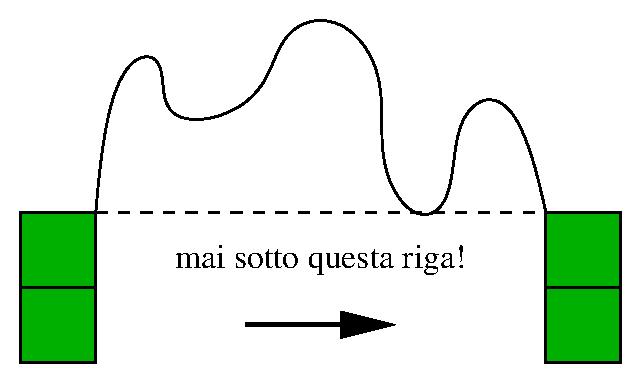
\epsfig{file = russe2.eps, width = 9cm}
\end{center}
\caption{L'esecuzione del bytecode Kitten generato per un comando non deve modificare lo stack degli operandi iniziale.}
  \label{fig:russian2}
\end{figure}
%
La generazione del bytecode per un comando Kitten \`e
formalizzata tramite una funzione $\gen{\_}:\mathtt{absyn.Command}\mapsto
\mathtt{translate.CodeBlock}\mapsto\mathtt{translate.CodeBlock}$.
Dato un comando $\mathit{com}$
e una continuazione $\beta$, il codice $\gen{\mathit{com}}(\beta)$
dovr\`a essere del bytecode Kitten che esegue il comando
$\mathit{com}$ e poi continua eseguendo la continuazione $\beta$.
Il codice generato per eseguire i comandi deve essere tale da
lasciare intatti i valori iniziali sullo stack degli operandi.
Si tratta esattamente dello stesso vincolo imposto al codice generato per
le espressioni nella Sezione~\ref{sec:expressions_bytecode_generation}.
In tal caso si chiedeva per\`o anche
che il valore dell'espressione fosse aggiunto
in cima allo stack degli operandi. Dal momento che i comandi non calcolano
alcun valore, non esiste per essi tale secondo vincolo. Il comportamento
del bytecode generato per i comandi sar\`a quindi come mostrato in
Figura~\ref{fig:russian2}.

\begin{figure}[t]
{\scriptsize
\begin{align*}
  \gen{\_}:\mathtt{absyn.Command}&\mapsto(\mathtt{translate.CodeBlock}\mapsto\mathtt{translate.CodeBlock})\\
  \mbox{}\\
  \gen{\mathtt{Skip()}}(\beta)=\beta\qquad&
    \gen{\mathtt{LocalScope(\mathit{body})}}(\beta)=
    \gen{\mathit{body}}(\beta)\\
  \gen{\mathtt{Return(\mathit{returned})}}(\beta)&=
    \begin{cases}
      \fbox{$\mathtt{return\ void}$} &
        \text{se $\mathit{returned}=\mathtt{null}$}\\
      \gen{\mathit{returned}}\left(\fbox{$\mathtt{return\ \tau}$}\right) &
        \text{se $\mathit{returned}\not=\mathtt{null}$ e
              ha tipo statico $\tau$}\\
    \end{cases} \\
  \gen{\mathtt{IfThenElse(\mathit{condition},\mathit{then},\mathit{else})}}
    (\beta)&=\gentest{\mathit{condition}}
      (\gen{\mathit{then}}(\beta))(\gen{\mathit{else}}(\beta))\\
  \gen{\mathtt{LocalDeclaration(\mathit{type},\mathit{name},
     \mathit{initialiser})}}(\beta)&=
       \gentwo{\tau}{\mathit{initialiser}}
        \left(\fbox{$\mathtt{store}\ \mathit{num}\ \mathtt{of\ type}\ \tau$}
        \to\beta\right)\\
  \text{dove $\tau$ \`e il tipo semantico di $\mathit{type}$} &
    \text{ e $\mathit{num}$ \`e il numero progressivo della variabile
    $\mathit{name}$}\\
  \gen{\mathtt{MethodCallCommand(\mathit{receiver},\mathit{name},
    \mathit{actuals})}}(\beta)&=\begin{cases}
    \gen{\mathit{receiver}}\left(\gentwo{\vec{t}}{\mathit{actuals}}
    \left(\fbox{$\mathtt{virtualcall}\ \mathit{method}$}
    \to\beta\right)\right) \\
    \quad\text{se $t'=\mathtt{void}$}\\
    \mbox{}\\
    \gen{\mathit{receiver}}\left(\gentwo{\vec{t}}{\mathit{actuals}}
    \left(\fbox{$\begin{array}{l}
      \mathtt{virtualcall}\ \mathit{method}\\
      \mathtt{pop}\ t'
    \end{array}$}
    \to\beta\right)\right)\\
    \quad\text{altrimenti}
  \end{cases} \\
  \text{dove $\mathit{method}=\kappa.\mathtt{m}(\vec{t}):t'$
        \`e il}&
  \text{ metodo identificato dall'analisi semantica
        (Figura~\ref{fig:analysis_expressions2})}\\
  \gen{\mathtt{Assignment(\mathit{lvalue},\mathit{rvalue})}}(\beta)&=
    \gamma^\mathit{before}\inter{\mathit{lvalue}}
    \left(\gentwo{\tau}{\mathit{rvalue}}
    (\gamma^\mathit{after}\inter{\mathit{lvalue}}(\beta))
    \right) \\
  \text{dove $\tau$ \`e il tipo}& \text{ statico di $\mathit{lvalue}$}\\
  \gen{\mathtt{While(\mathit{condition},\mathit{body})}}(\beta)&=
    \underbrace{\fbox{$\mathtt{nop}$}}_\mathit{pivot}
    \to\gentest{\mathit{condition}}(\gen{\mathit{body}}(\mathit{pivot}))
    (\beta)\\
  \gen{\mathtt{For(\mathit{initialiser},\mathit{condition},\mathit{update},
    \mathit{body})}}(\beta)&=
    \gen{\mathit{initialiser}}
    \left(\underbrace{\fbox{$\mathtt{nop}$}}_\mathit{pivot}\to
    \gentest{\mathit{condition}}\left(\gen{\mathit{body}}\left(
    \gen{\mathit{update}}(\mathit{pivot})
    \right)\right)(\beta)
    \right)
\end{align*}
}
\caption{La funzione $\gen{\_}$ che genera il bytecode Kitten che esegue i comandi.}
  \label{fig:commands_generation}
\end{figure}

La Figura~\ref{fig:commands_generation} mostra il codice generato per i
comandi Kitten. Commentiamo tali regole di compilazione.
%
\begin{description}
\item[\underline{$\mathtt{Skip()}$}.] Questo comando non genera alcun
  bytecode e quindi la sua compilazione restituisce la continuazione $\beta$.
\item[\underline{$\mathtt{LocalScope(\mathit{body})}$}.]
  L'esecuzione di uno scope locale consiste nell'esecuzione del suo corpo.
  Conseguentemente, la sua compilazione \`e, ricorsivamente, la compilazione
  del suo corpo.
\item[\underline{$\mathtt{Return(\mathit{returned})}$}.]
  L'istruzione di ritorno da metodo viene tradotta in un bytecode
  $\mathtt{return}$ per il tipo del valore ritornato, se esiste.
  In tal caso occorre prima compilare l'espressione il cui
  valore va ritornato.
  Si noti che la continuazione $\beta$ \`e scartata poich\'e
  l'esecuzione di un metodo termina col ritorno al chiamante.
\item[\underline{$\mathtt{IfThenElse(\mathit{condition},\mathit{then},
  \mathit{else})}$}.]
  La compilazione del condizionale comincia con la compilazione come
  test della sua guardia (Sezione~\ref{subsec:conditional_generation}).
  Le due continuazioni della guardia sono, rispettivamente, la compilazione
  del ramo \texttt{then} e del ramo \texttt{else} del condizionale,
  seguite dalla continuazione $\beta$ del condizionale.
\item[\underline{$\mathtt{LocalDeclaration(\mathit{type},\mathit{name},
  \mathit{initialiser})}$}.]
  La compilazione della dichiarazione di una variabile locale, con
  inizializzazione, \e del codice che
  valuta l'inizializzatore e ne lascia il valore in cima allo stack,
  da cui \`e poi rimosso e scritto dentro alla variabile tramite un bytecode
  $\mathtt{store}$. Si noti che il numero
  $\mathit{num}$ della variabile \`e stato assegnato al momento dell'analisi
  semantica.
\item[\underline{$\mathtt{MethodCallCommand(\mathit{receiver},
  \mathit{name},\mathit{actuals})}$}.]
  La compilazione del comando di invocazione di metodo \`e
  quasi identica a quella che abbiamo visto per l'espressione di
  invocazione di metodo (Figura~\ref{fig:expressions_generation}).
  La differenza \`e che qui \`e possibile invocare anche un metodo che
  ritorna \texttt{void}. Inoltre, dal momento che non dobbiamo modificare
  lo stack degli operandi (Figura~\ref{fig:russian2}), rimuoviamo
  il valore di ritorno di un metodo non \texttt{void} tramite un
  bytecode \texttt{pop}.
\item[\underline{$\mathtt{Assignment(\mathit{lvalue},\mathit{rvalue})}$}.]
  La compilazione di un assegnamento di $\mathit{rvalue}$ ad
  $\mathit{lvalue}$ \e ottenuta come in Figura~\ref{fig:passive_leftvalues}.
\item[\underline{$\mathtt{While(\mathit{condition},\mathit{body})}$}.]
  Il codice generato per un ciclo \texttt{while} \`e la compilazione
  condizionale della sua guardia (Sezione~\ref{subsec:conditional_generation}),
  usando come due continuazioni quella stessa del \texttt{while}, per
  il caso in cui la guardia \`e falsa, e la compilazione del
  corpo per il caso in cui la guardia \`e vera. Si noti che la
  continuazione fornita alla compilazione del corpo \`e un blocco
  \textit{pivot}
  che continua con la compilazione condizionale della guardia stessa,
  in modo che dopo l'esecuzione del corpo del \texttt{while} si passi
  a valutare di nuovo la guardia del ciclo.
\item[\underline{$\mathtt{For(\mathit{initialiser},\mathit{condition},
  \mathit{update},\mathit{body})}$}.]
  Il codice generato per un ciclo \texttt{for} comincia con il codice
  che esegue il comando di inizializzazione, seguito da un blocco
  \textit{pivot} legato alla compilazione condizionale della guardia
  del \texttt{for} (Sezione~\ref{subsec:conditional_generation}).
  Le due continuazioni passate a tale compilazione condizionale sono
  la continuazione $\beta$ del \texttt{for}, per il caso in cui la
  guardia \`e falsa, e la compilazione dell'\textit{update} e del corpo
  del ciclo per il caso in cui la guardia \`e vera. Si noti che la
  continuazione usata per la compilazione del corpo \`e il \textit{pivot},
  in modo che dopo l'esecuzione del corpo del \texttt{for} si torni a valutare
  la guardia del ciclo.
\end{description}

L'implementazione della generazione del codice per i comandi \`e ottenuta
aggiungendo i seguenti metodi ad \texttt{absyn/Command.java}:
%
\begin{verbatim}
  public final CodeBlock translate(CodeBlock continuation) {
    if (next != null) continuation = next.translate(continuation);
    return translate$0(continuation);
  }

  protected abstract CodeBlock translate$0(CodeBlock continuation);
\end{verbatim}
%
Il primo si occupa del lavoro comune a tutti i comandi, che consiste
nel compilare il comando che potrebbe seguire ottenendo la continuazione
da passare al metodo \texttt{translate\$0()}.
Quest'ultimo si occupa del lavoro specifico a ogni comando.
Esso implementa le regole in Figura~\ref{fig:commands_generation}.

Vediamo alcuni esempi di definizione di \texttt{translate\$0()} in alcune
delle sottoclassi della classe \texttt{absyn/Command.java}.
Dentro \texttt{absyn/LocalScope.java} definiamo
%
\begin{verbatim}
  protected CodeBlock translate$0(CodeBlock continuation) {
    return body.translate(continuation);
  }
\end{verbatim}
% $
consistentemente con la Figura~\ref{fig:commands_generation}.
In \texttt{absyn/IfThenElse.java} definiamo
%
\begin{verbatim}
  protected CodeBlock translate$0(CodeBlock continuation) {
    return condition.translateAsTest
      (then.translate(continuation),else.translate(continuation));
  }
\end{verbatim}
% $
ancora una volta questo rispecchia la formalizzazione in
Figura~\ref{fig:commands_generation}.

L'implementazione delle regole
per il \texttt{while} e il \texttt{for} richiedono di creare
\emph{prima} il \textit{pivot} in modo da poterlo passare come continuazione,
rispettivamente, alla compilazione del \textit{body} o
dell'\textit{update} del ciclo. Alla fine si lega il blocco \textit{pivot} con
il suo successore, chiudendo il ciclo. Ecco per esempio il generatore di codice
inserito dentro \texttt{absyn/For.java}:
%
\begin{verbatim}
  protected CodeBlock translate$0(CodeBlock continuation) {
    CodeBlock pivot = new CodeBlock();
    CodeBlock test = condition.translateAsTest
      (body.translate(update.translate(pivot)),continuation);
    pivot.linkTo(test);
    return initialisation.translate(test);
  }
\end{verbatim}
%$
\javatip{
Si noti che il blocco \emph{pivot} va creato prima di usarlo come
continuazione per la compilazione di \texttt{update}, nel caso del
comando \texttt{for}. Sarebbe sbagliato dichiarare la variabile
\texttt{pivot} e creare il blocco \emph{pivot} subito prima della
chiamata a \texttt{linkTo()}: l'\texttt{update} si troverebbe con una
continuazione pari a \texttt{null}!}

La generazione del bytecode Kitten per un metodo o costruttore \`e
semplicemente la generazione del bytecode Kitten per
il loro corpo, che essendo un comando segue
le regole in Figura~\ref{fig:commands_generation}.
Come continuazione di tale compilazione si usa il blocco
\[
  \overline{\beta}=\fbox{$\mathtt{return\ void}$}~.
\]
In questo modo abbiamo la garanzia che, nel bytecode che viene generato,
ogni percorso di esecuzione
all'interno di un metodo che ritorna \texttt{void} o all'interno di un
costruttore termina sempre con un'istruzione \texttt{return\ void}, anche
nei casi in cui il comando \texttt{return} \`e stato lasciato
sottointeso dal programmatore. Si noti che nel caso in cui fossimo
dentro un metodo che non ritorna \texttt{void} allora tale continuazione
verrebbe sistematicamente scartata dalla regola per
il comando Kitten \texttt{return} in Figura~\ref{fig:commands_generation}, dal
momento abbiamo la garanzia che, in tal caso, ogni percorso di
esecuzione all'interno del metodo termina gi\`a con un comando
\texttt{return} esplicito (Sezione~\ref{sec:dead_code}).
%
\begin{exercise}\label{ex:conditional_expression_compilation}
Si parta dalla sintassi astratta dell'espressione condizionale definita
nell'Esercizio~\ref{ex:conditional_expression} e si scriva la sua
funzione $\gamma$ di compilazione, implementandola poi in Java.
\end{exercise}
%
\begin{exercise}\label{ex:do_while_compilation}
Si definisca la sintassi astratta di un comando
\texttt{do}\ldots\texttt{while} e si dia quindi la sua funzione $\gamma$
di compilazione, implementandola poi in Java.
\end{exercise}
%
\begin{exercise}\label{ex:switch_compilation}
Si parta dalla sintassi astratta del comando \texttt{switch} definito
nell'Esercizio~\ref{ex:switch} e si definisca la sua funzione $\gamma$ di
compilazione, implementandola poi in Java.
\end{exercise}
%
\begin{exercise}\label{ex:break_continue_continuation}
Quali problemi vedete per definire la compilazione dei comandi
\texttt{break} e \texttt{continue} dell'Esercizio~\ref{ex:break_continue}?
Come pensate di poter modificare lo schema di compilazione per
continuazioni in modo da poter compilare tali due comandi?
\end{exercise}
